% updated April 2002 by Antje Endemann
% Based on CVPR 07 and LNCS, with modifications by DAF, AZ and elle, 2008 and AA, 2010, and CC, 2011; TT, 2014; AAS, 2016; AAS, 2020; TH, 2022

\documentclass[runningheads]{llncs}
% \documentclass{article}

\usepackage{graphicx}
\usepackage{hyperref}
\hypersetup{
    colorlinks=true,
    linkcolor=black,
    filecolor=magenta,      
    urlcolor=cyan,
    pdftitle={Overleaf Example},
    pdfpagemode=FullScreen,
    }
\usepackage{tikz}
\usepackage{comment}
\usepackage{amsmath,amssymb} % define this before the line numbering.
\usepackage{color}
\usepackage{setspace}
\usepackage{appendix}
\usepackage{subfig}
\usepackage{fancyvrb}
\DefineVerbatimEnvironment{SmallVerbatim}{Verbatim}{fontsize=\small}

\usepackage[accsupp]{axessibility}  % Improves PDF readability for those with disabilities.
\usepackage[width=122mm,left=12mm,paperwidth=146mm,height=193mm,top=12mm,paperheight=217mm]{geometry}

% \renewcommand{\labelitemi}{$\bullet$}


\begin{document}

\pagestyle{headings}
\mainmatter
% \def\ECCVSubNumber{100}  % Insert your submission number here



\author{Ouyang Mingyu, Lin Liangtao, Li Zeyun, Tang Zheng, Zhou Yuhao}

\institute{DSA 5104 Final Project\\Group 24}


% \addtocontents{toc}{\protect\setcounter{tocdepth}{-1}}

\title{\textit{Yelp Insight}: \\A Comprehensive Platform for Customers, Business Owners, and Administrators} % Replace with your title

\maketitle

% \addtocontents{toc}{\protect\setcounter{tocdepth}{3}} % Reset TOC depth

\begin{abstract}
In this project, we proposed a comprehensive data platform, namely \textit{Yelp Insight}, for customers, business owners, and administrators. The highlights of our project can be concluded as follows: 1. We added more than 6,000 entries of Yelp data using the customized web crawler, and 180,000 rows of features via large language model generation techniques. 2. We carefully explored the characteristics of our Yelp dataset and presented many interesting insights into Yelp. 3. We provide more than 100 querying methods via the combination of our 16 basic queries and flexible parameters, which could cover a wide range of demands from customers, business owners, and platform administrators. 4. We built a demo website that can provide data access services via a non-coding interface. The code and demo of our project will be available at: \url{https://github.com/Linlt-leon/Yelp-Insight}.
\end{abstract}


%******************

\setcounter{tocdepth}{3}

\begin{spacing}{1.3}
\tableofcontents
\end{spacing}

\newpage  % This command starts a new page



\section{Introduction}

\subsection{Project Overview}

The objective of our proposed \textit{YELP Insight} project is to dive into the methodologies of data management and retrieval, focusing on simulating the practical applications in real-world scenarios via the given YELP dataset \cite{YelpDataset}. This mainly involves a sequence of critical tasks: data collection, processing, storage, and access.

\textbf{Data Collection:} The initial collection step involves gathering relevant data from diverse sources. For further emphasizing comprehensiveness, in addition to the original dataset, we also: 1. crawled data from the current date yelp.com, 2. generated complicated data attributes via the large language models. This step forms the foundation upon which subsequent processes are built.

\textbf{Data Processing:} Once collected, the raw data undergoes some preprocessing operations. This transforms the massive data into a structured format, making it suitable for the following analysis and storage. Processing includes data cleaning, file splitting, and preparing the data for further use.

\textbf{Data Storage:} The data is then stored in our databases. We will explore two primary storage methods: traditional SQL databases (MySQL \cite{MySQL}) and NoSQL databases (MongoDB \cite{MongoDB}). This dual approach allows for a comparative understanding of different storage models and their characteristics for various data types.

\textbf{Data Access:} The accessing stage focuses on retrieving and utilizing the stored data effectively. This project developed efficient retrieval methods, ensuring that data is accessible and usable in our desired applications. This involves the creation of optimized SQL and NoSQL queries, and we also made comparisons of their performances.

\textbf{Applications:} The \textit{YELP Insight} project is designed to fit these concepts into real-world applications, providing a comprehensive view of data management in a real-world setting. This hands-on approach ensures that the theoretical knowledge gained is grounded in practical, applicable skills, essential for tackling real-world data challenges.



\subsection{Collaboration and Contributions}

\begin{itemize}
    \item Ouyang Mingyu: group leader, overall engagement
    \item Lin Liangtao: data generation
    \item Li Zeyun: data storage
    \item Tang Zheng: data access
    \item Zhou Yuhao: data analysis and cleaning

\end{itemize}

\clearpage

\section{Data Analysis}

According to the compressed JSON files provided by Dr. Yang, we proceed data understanding and cleaning in Python for YELP data. 

\subsection{Understanding the original YELP Dataset}
The \textit{business} dataset is of length 150346 and contains 14 attributes, which are \textit{business\_id}, \textit{name}, \textit{address} of each business, together with the \textit{city}, \textit{state}, \textit{postal\_code}, \textit{latitude}, \textit{longitude} of a particular business, as well as its \textit{stars} rating which has been rounded to half-stars, with the collective \textit{review\_count}. Also, a binary indicator of whether a particular business \textit{is\_open} or not is also included. The embedded attribute \textit{attributes} containing miscellaneous \textbf{binary} topics about whether a business \textit{BusinessAcceptsCreditCards}, the method of parkings available \textit{BikeParking}, \textit{BusinessParking} et cetera are also stored. Also, an informative array indicating what kinds of \textit{categories} a business belongs to, and the opening \textit{hours} for it is also included in the dataset. \\
For data types, we see \textit{business\_id} (22 character unique), \textit{name}, \textit{address}, \textit{city}, \textit{state}, \textit{postal\_code}, \textit{categories} are of \textbf{string} (or an array of \textbf{strings}) type, while \textit{latitude}, \textit{longitude}, \textit{stars} are of \textbf{float} type, \textit{review\_count} and \textit{is\_open} (0 or 1 for closed or open, respectively) is of \textbf{integer} type, and \textit{attributes} (key business attribute to a binary value) and \textit{hours} (key day to value hours using 24-hour clock) are of the embedded \textbf{object} type. \\
After verification, we find that \textbf{the Primary Key of \textit{business} is \textit{business\_id}}. \\

The \textit{checkin} dataset is of length 131930 and contains 2 attributes, which are \textit{business\_id}, which is a \textbf{Foreign Key} mapped to \textit{business\_id} in \textit{business} dataset, and the \textit{date} for each checkin at the business. \\
For data types, we see \textit{business\_id} is of 22 character unique \textbf{string} type, and \textit{date} is also of type \textit{string}, but  is a comma-separated list of strings, each with format YYYY-MM-DD HH:MM:SS. \\
After verification, we find that \textbf{the Primary Key of \textit{checkin} is \textit{business\_id}}. \\

The \textit{review} dataset is of length 6990280 and contains 9 attributes, which are \textit{review\_id} for each review, \textit{user\_id} for the user that posts a review, which is a \textbf{Foreign Key} mapped to \textit{user\_id} in \textit{user} dataset (discuss later), \textit{business\_id} for the business that a user posts a review on, which is a \textbf{Foreign Key} mapped to \textit{business\_id} in \textit{business} dataset, and the \textit{stars} rating which has been rounded to full-stars that the user gave to a particular business, the number of \textit{useful}, \textit{funny}, \textit{cool} votes received, respectively, as well as the textual \textit{text} represents the full given review itself from a user, also the \textit{date} of the review being posted was given.\\
For data types, we see \textit{review\_id} is of 22 character unique \textbf{string} type, and \textit{user\_id}, \textit{business\_id} and \textit{text} are also of type \textit{string}. The attribute \textit{date} is of a special \textit{string} type, for which each of them holds the format of YYYY-MM-DD HH:MM:SS, while the attributes \textit{stars}, \textit{useful}, \textit{funny}, \textit{cool} are of \textit{integer} type. \\
After verification, we find that \textbf{the Primary Key of \textit{review} is \textit{review\_id}}. \\

The \textit{tip} dataset is of length 908915 and contains 5 attributes, which are \textit{user\_id} for each customer given an amount of tips, which is a \textbf{Foreign Key} mapped to \textit{user\_id} in \textit{user} dataset (discuss later). The attribute \textit{business\_id} for the business of a user that gave some tips to, which is a \textbf{Foreign Key} mapped to \textit{business\_id} in \textit{business} dataset, and the full textual script of \textit{text} for the tips given, as well as the exact time 
 of the \textit{date} that a tip was written, together with the number of \textit{compliment\_count} it has. \\
For data types, we see \textit{user\_id} and \textit{business\_id} are of 22 character \textbf{string} type and \textit{text} is of normal \textbf{string} type. The attribute \textit{date} is of a special \textit{string} type, for which each of them holds the format of YYYY-MM-DD HH:MM:SS, while \textit{compliment\_count} is of \textit{integer} type. Even after data cleaning (discuss later), we find that \textbf{there is no specific Primary Key of \textit{tip} and we may need to create one}. \\

The \textit{user} dataset is of length 1987897 and contains 22 attributes, which are \textit{user\_id} for a particular user, \textit{name} for the user's first name, and the \textit{review\_count} which indicates the number of reviews a user has written. The \textit{yelping\_since} attribute shows the exact date and time of when the user joined Yelp. Also, \textit{tip} contains the number of \textit{useful}, \textit{funny}, \textit{cool} votes sent by a specific user, respectively, as well as the \textit{elite} indicator that in which year(s) a user was badged as an elite. \textit{friends} represents the an array of the user's friend presented as \textit{user\_id} forms, as well as the \textit{fans} that user has. Subsequently, the \textit{average\_stars} records the average rating of all reviews that a user has given so far. Eventually, the attributes \textit{compliment\_hot}, \textit{compliment\_more}, \textit{compliment\_profile}, \textit{compliment\_cute}, \textit{compliment\_list}, \textit{compliment\_note}, \textit{compliment\_plain}, \textit{compliment\_cool}, \textit{compliment\_funny}, \textit{compliment\_writer}, \textit{compliment\_photos} specifies the number of different types of compliments which is self-explainable, received by the user. \\ 
For data types, we see \textit{user\_id} is of 22 character unique \textbf{string} type, and \textit{name} is also of type \textit{string}. The attribute \textit{yelping\_since} is of a special \textit{string} type, for which each of them holds the format of YYYY-MM-DD HH:MM:SS, and the attribute \textit{friends} is an array of \textit{strings}, while the attributes \textit{review\_count}, \textit{useful}, \textit{funny}, \textit{cool}, \textit{fans}, \textit{elite} (array of \textit{integers}), \textit{compliment\_hot}, \textit{compliment\_more}, \textit{compliment\_profile}, \textit{compliment\_cute}, \textit{compliment\_list}, \textit{compliment\_note}, \textit{compliment\_plain}, \textit{compliment\_cool}, \textit{compliment\_funny}, \textit{compliment\_writer}, \textit{compliment\_}\\
-\textit{photos} are of \textit{integer} type. Finally, the attribute \textit{average\_stars} is of \textit{float} type. \\
After verification, we find that \textbf{the Primary Key of \textit{user} is \textit{user\_id}}. 

\subsection{Data Cleaning and Statistical Analysis}
Through rectifying incorrect, incomplete, and duplicated data, we see that there are 13744, 103, and 23223 missing values in attributes \textit{attributes}, \textit{categories} and \textit{hours} in \textit{business} dataset, and 67 duplicates in \textit{tip} dataset. After data cleaning, we see the \textit{business} dataset contains 117618 rows and \textit{tip} dataset is of length 908848. 

After data cleaning, we perform Exploratory Data Analysis on meaningful attributes from the newly cleaned datasets \textit{business} and \textit{review}. \\
There are totally 86009 number of unique businesses collected in the dataset, for which \textbf{Starbucks} is ranked the top in the collection, and restaurant-related business seems to be the most popular business name for which we shall check later with attribute \textit{categories}. 

\begin{figure}[!h]
\centering
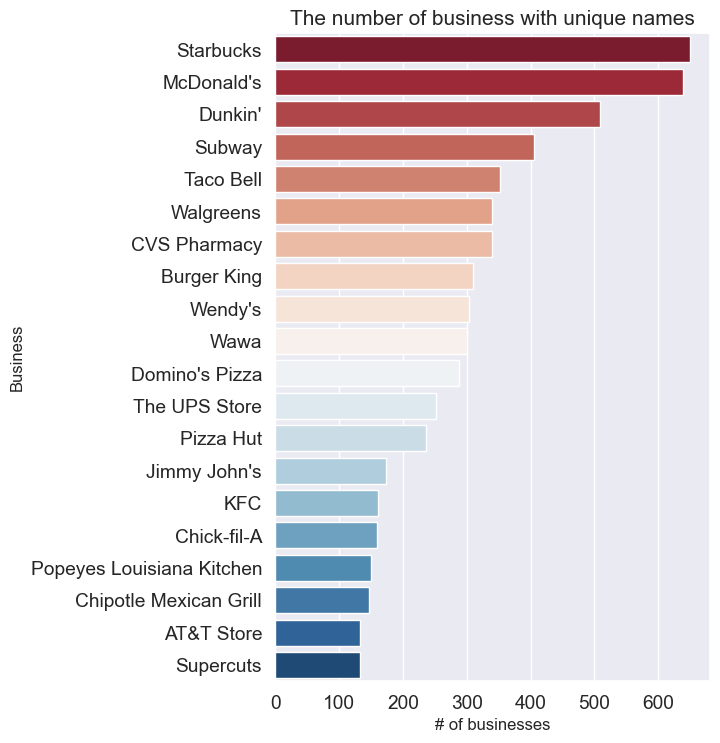
\includegraphics[height=8cm]{figs/name.png}
\caption{Top count of unique businesses}
\label{fig:name}
\end{figure}

Since the collective information \textit{city} and \textit{state} attributes provide are closely related with business counts, we may group them by each city and state to see top popular businesses for each city and state. We observe that there are 1261 city listed in the cleaned Yelp dataset and Philadelphia is the top of the city list in business listing in Yelp dataset followed by Tucson, Tampa etc. Meanwhile, there are 23 state listed, for which state PA is on the top of the state list. Interestingly, observing the full list of state rankings, there are almost half of states having very few business listing. 
\newpage
\begin{figure}[!h]
\centering
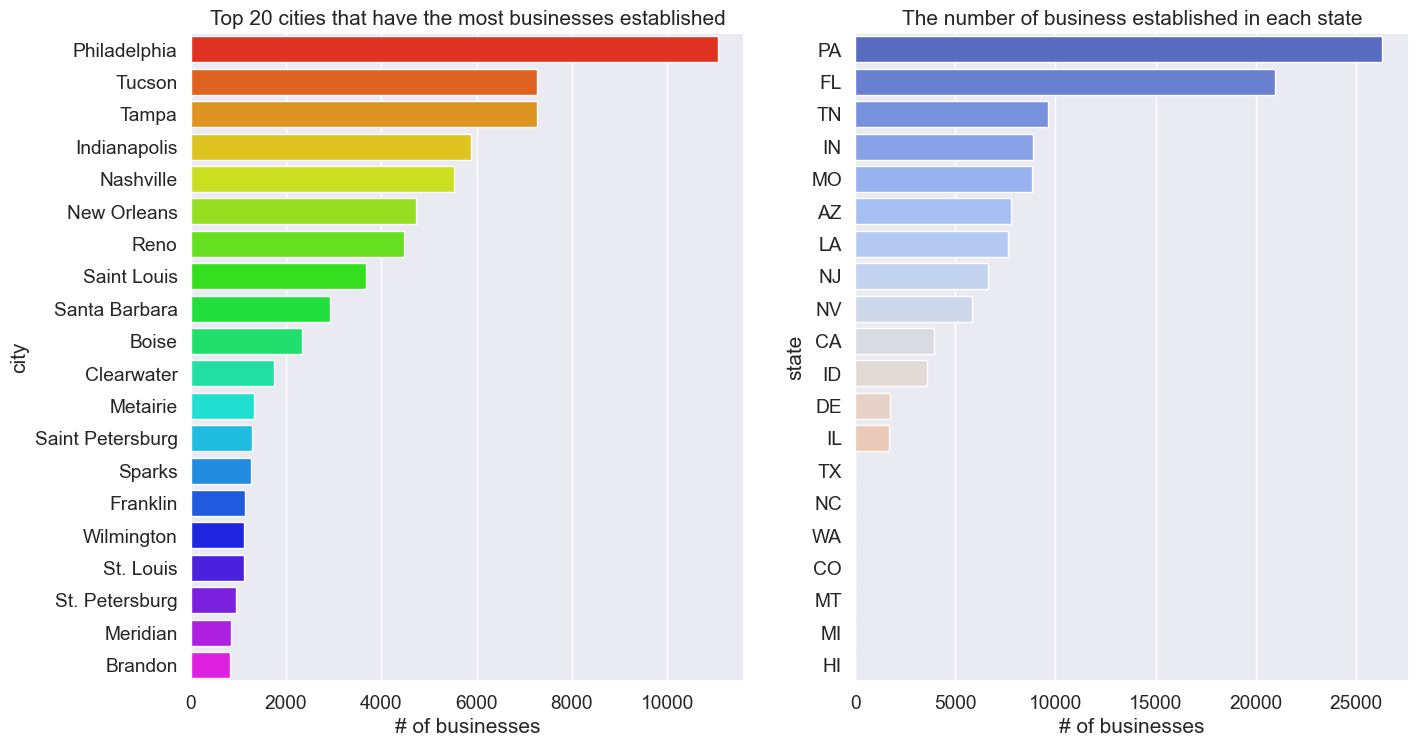
\includegraphics[height=6cm, width=12cm]{figs/citystate.png}
\caption{Top count of businesses in each city and state}
\label{fig:citystate}
\end{figure}

For geometric distribution of the businesses, we utilize \textit{latitude} and \textit{longitude} attributes, and view the plot from a satellite vision. 

\begin{figure}[!h]
\centering
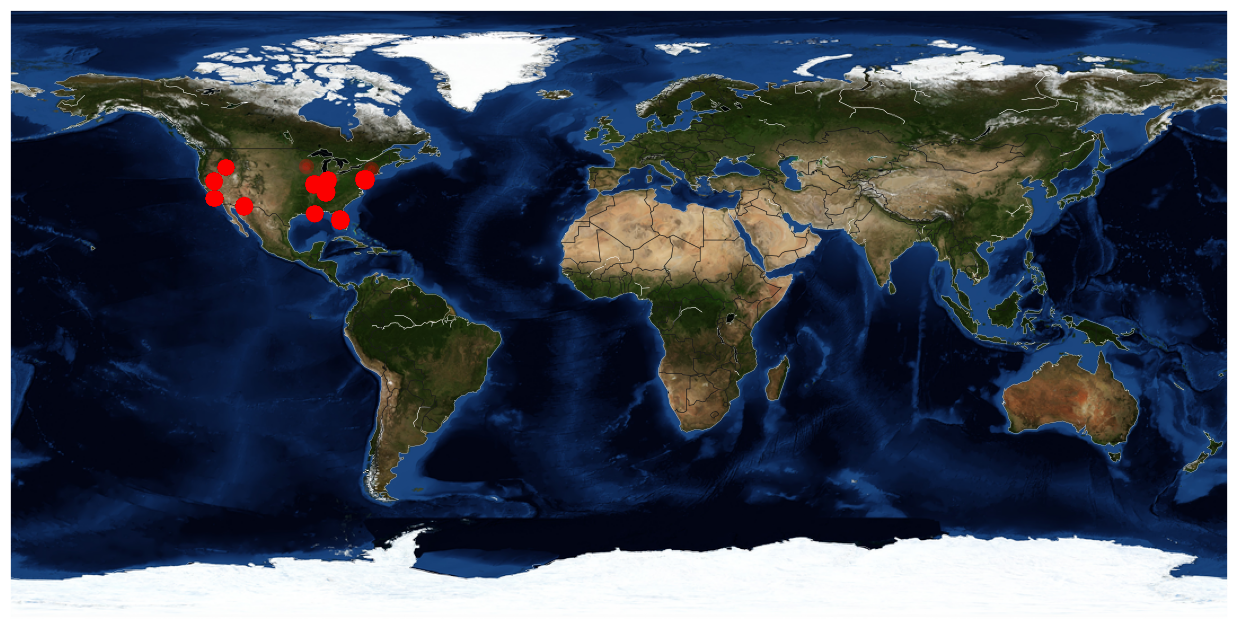
\includegraphics[height=6cm, width=12cm]{figs/latlongmap.png}
\caption{Satellite vision of businesses in each city and state}
\label{fig:latlongmap}
\end{figure}

To demonstrate the distribution of \textit{stars} rating which are half-stars ranging from 1 to 5, we collect the counts for individual \textit{stars} and use bar-plots. We see that most customers give 3.5, 4, and 4.5 stars to the businesses. 

\begin{figure}[!h]
\centering
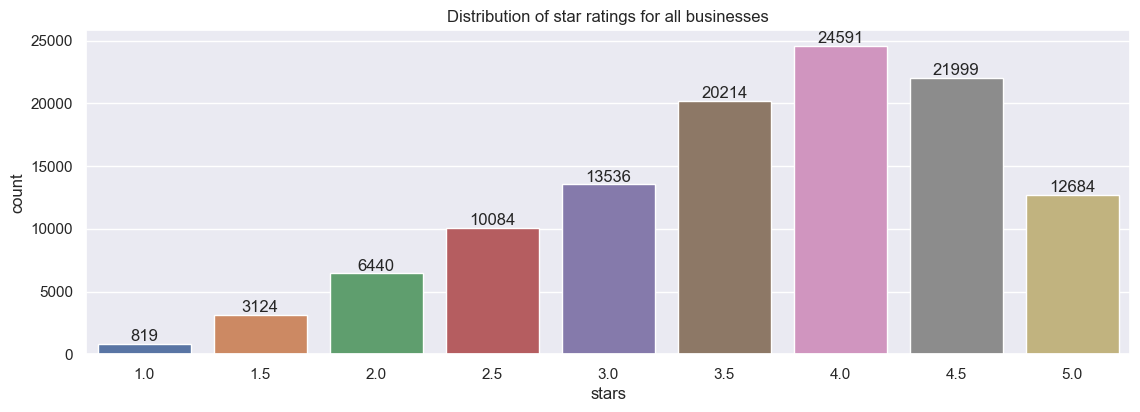
\includegraphics[width=12cm]{figs/stars.png}
\caption{Distribution of star ratings for all businesses}
\label{fig:stars}
\end{figure}

Now, we proceed with attribute pairs investigation and firstly look for businesses that received the most reviews counted globally which utilize attributes \textit{name} and \textit{review\_count} and find that \textbf{Starbucks} received the most reviews, where one shall not be surprised about the result since \textbf{Starbucks} has the most number of stores counted in the region of our interest. Based on the result, we calculate the mean of the review count for all businesses is 71, as well as the median of review count for them is 19. 

\begin{figure}[!h]
\centering
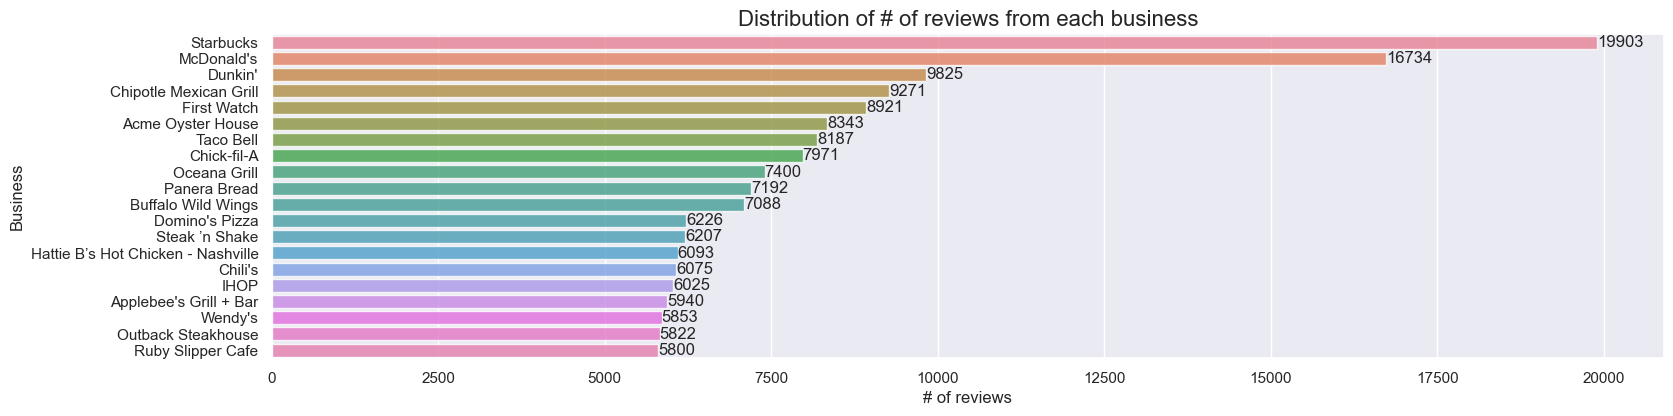
\includegraphics[width=12cm]{figs/reviewcounts.png}
\caption{Distribution of the number of reviews of each business}
\label{fig:reviewcounts}
\end{figure}

Based on inspiration to investigate cross-attribute pairs, we then look for businesses that received the most reviews counted in each city which utilize attributes \textit{city} and \textit{review\_count} and find that businesses in \textbf{Philadelphia} received the most reviews, where one shall not be surprised about the result since \textbf{Philadelphia} has the most number of businesses established in the region of our interest. Based on the result, we calculate the mean of the review count for businesses recorded in all cities is 4869, as well as the median of review count for them is 88. 

\begin{figure}[!h]
\centering
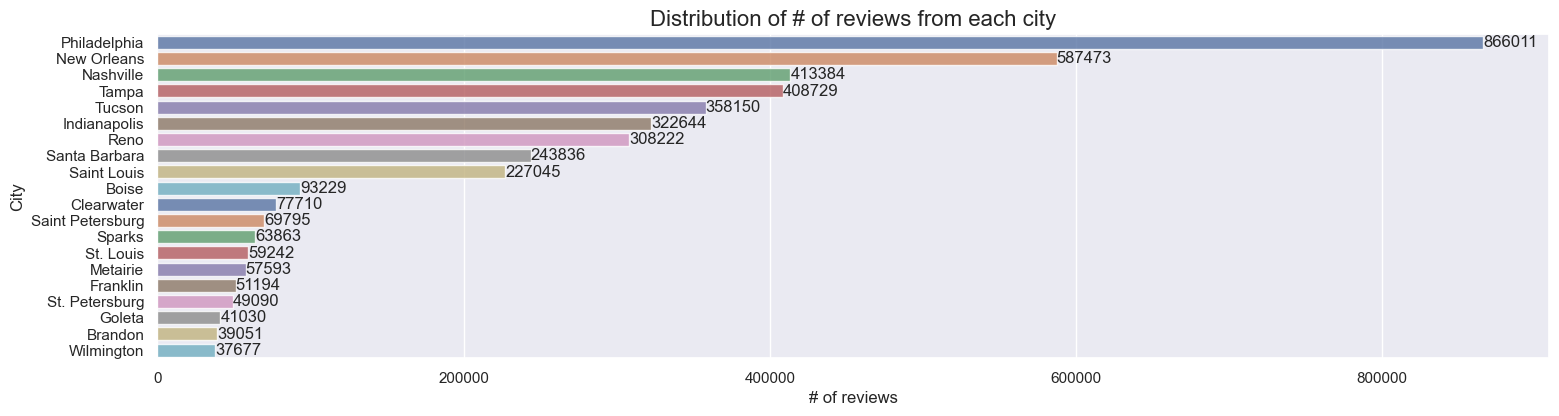
\includegraphics[width=12cm]{figs/citybusiness.png}
\caption{Distribution of the number of reviews from each city}
\label{fig:citybusiness}
\end{figure}

We then checked the proportion of businesses are still available utilizing the attribute \textit{is\_open} and find that 81\% of them are still open. \\

Finally, for \textit{business} dataset, we look into the embedded attribute \textit{categories} and would like to show its distribution. Just as we have claimed, restaurant-related business are the most popular, including \textit{Restorants}, \textit{Food}, \textit{Bars} and so on, for which we show the WordCloud of the category names since it contains string elements only. Meanwhile, for \textit{review} dataset, to analyse the textual attribute, we also use WordCloud of the \textit{text} and find that most text reviews are nouns about the place, food, order and service, verbs go, got, know, try, and a few adjectives love and amazing to express their appreciation for a particular business. The combined wordcloud figure is presented in figure\ref{fig:combinedwc}.


% \begin{figure}[!h]
% \centering
% 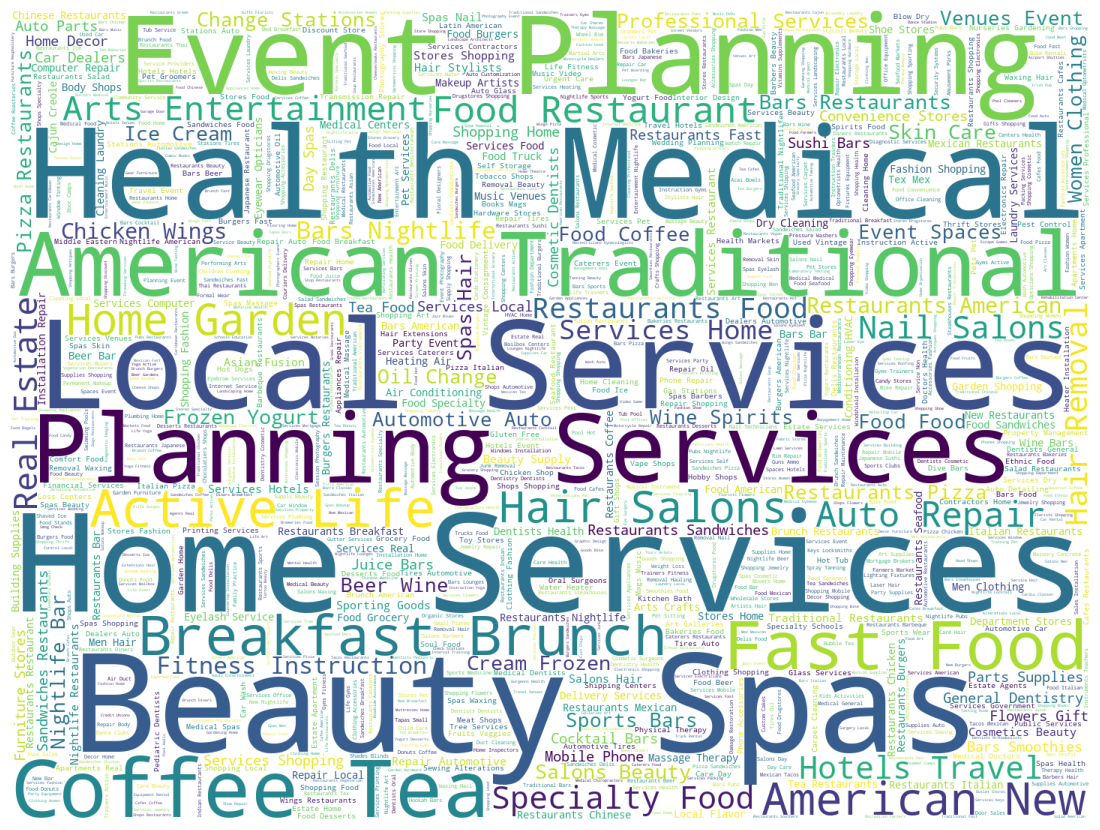
\includegraphics[height=6cm, width=8cm]{figs/categoriesWC.png}
% \caption{WordCloud of the categories}
% \label{fig:categorieswc}
% \end{figure}


% \begin{figure}[!h]
% \centering
% 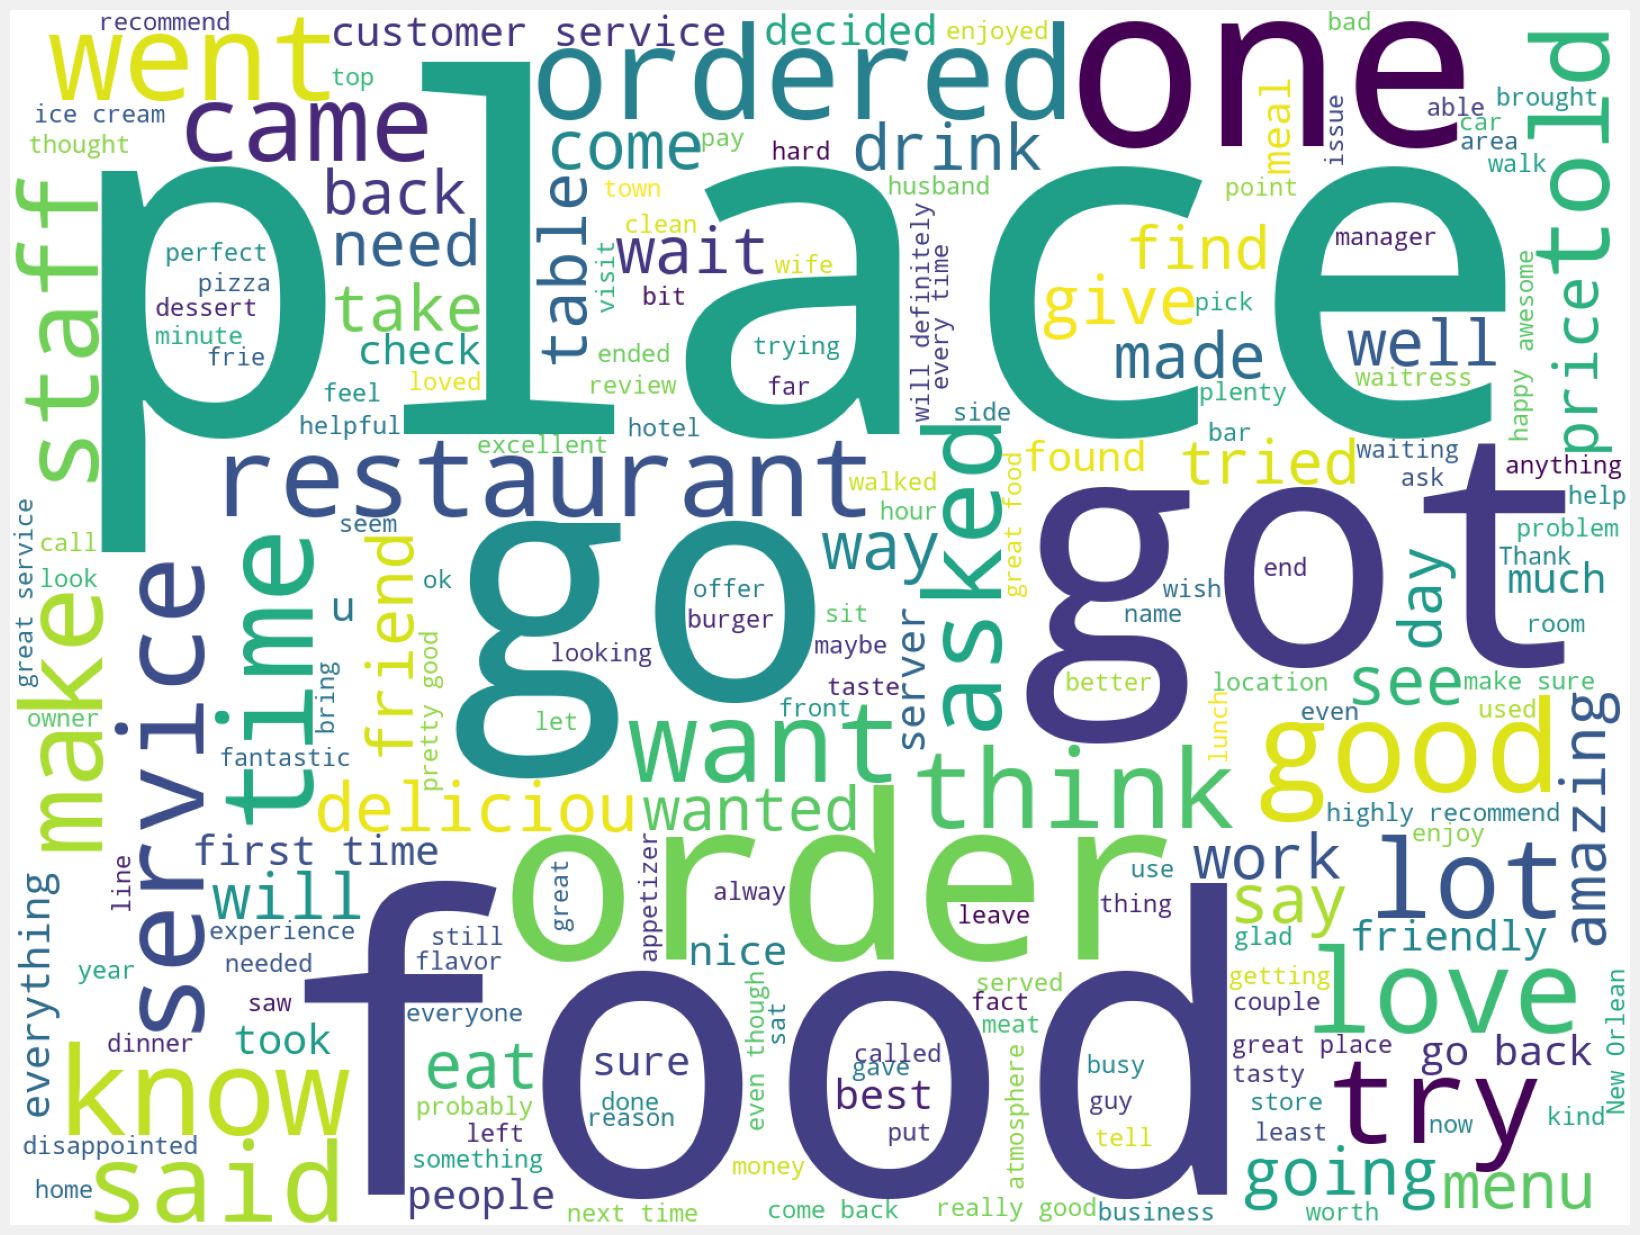
\includegraphics[height=6cm, width=8cm]{figs/reviewWC.png}
% \caption{WordCloud of the text reviews}
% \label{fig:reviewwc}
% \end{figure}



\begin{figure}[!h]
    \centering
    \subfloat[Categories]{
        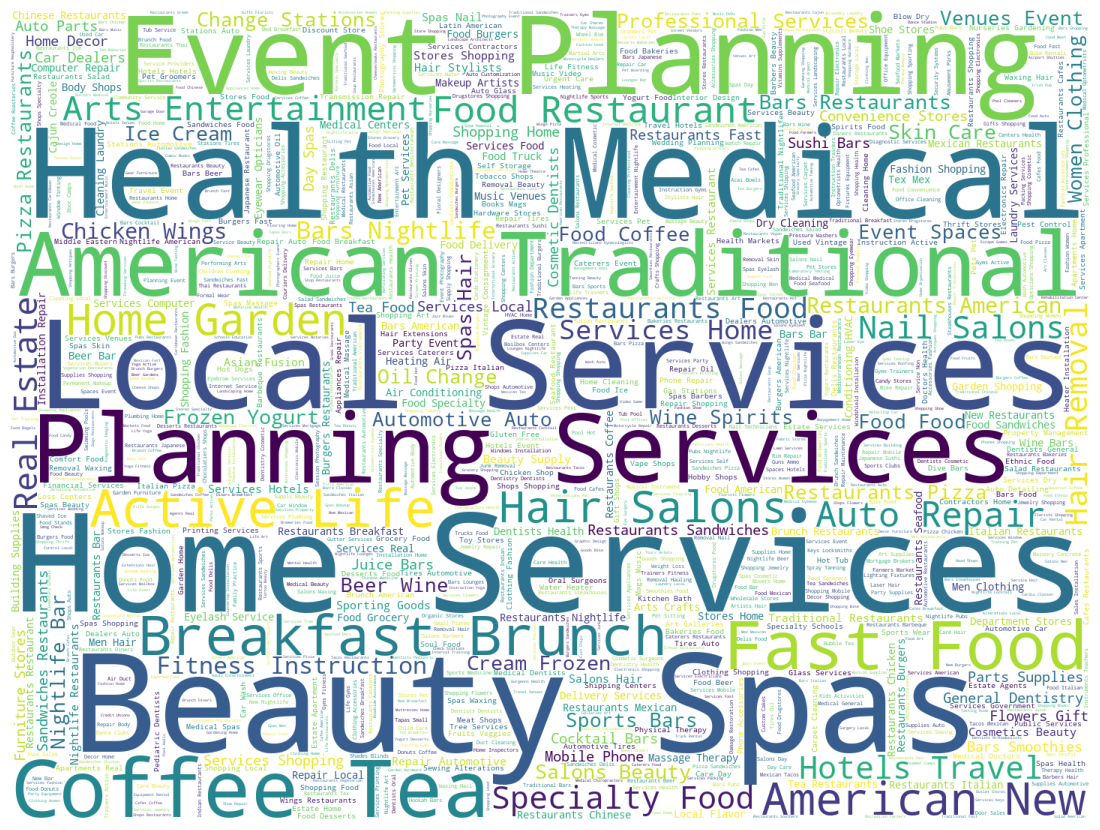
\includegraphics[width=0.47\textwidth]{figs/categoriesWC.png}
        \label{fig:categorieswc}
    }
    \hspace{0.07cm}
    \subfloat[Reviews]{
        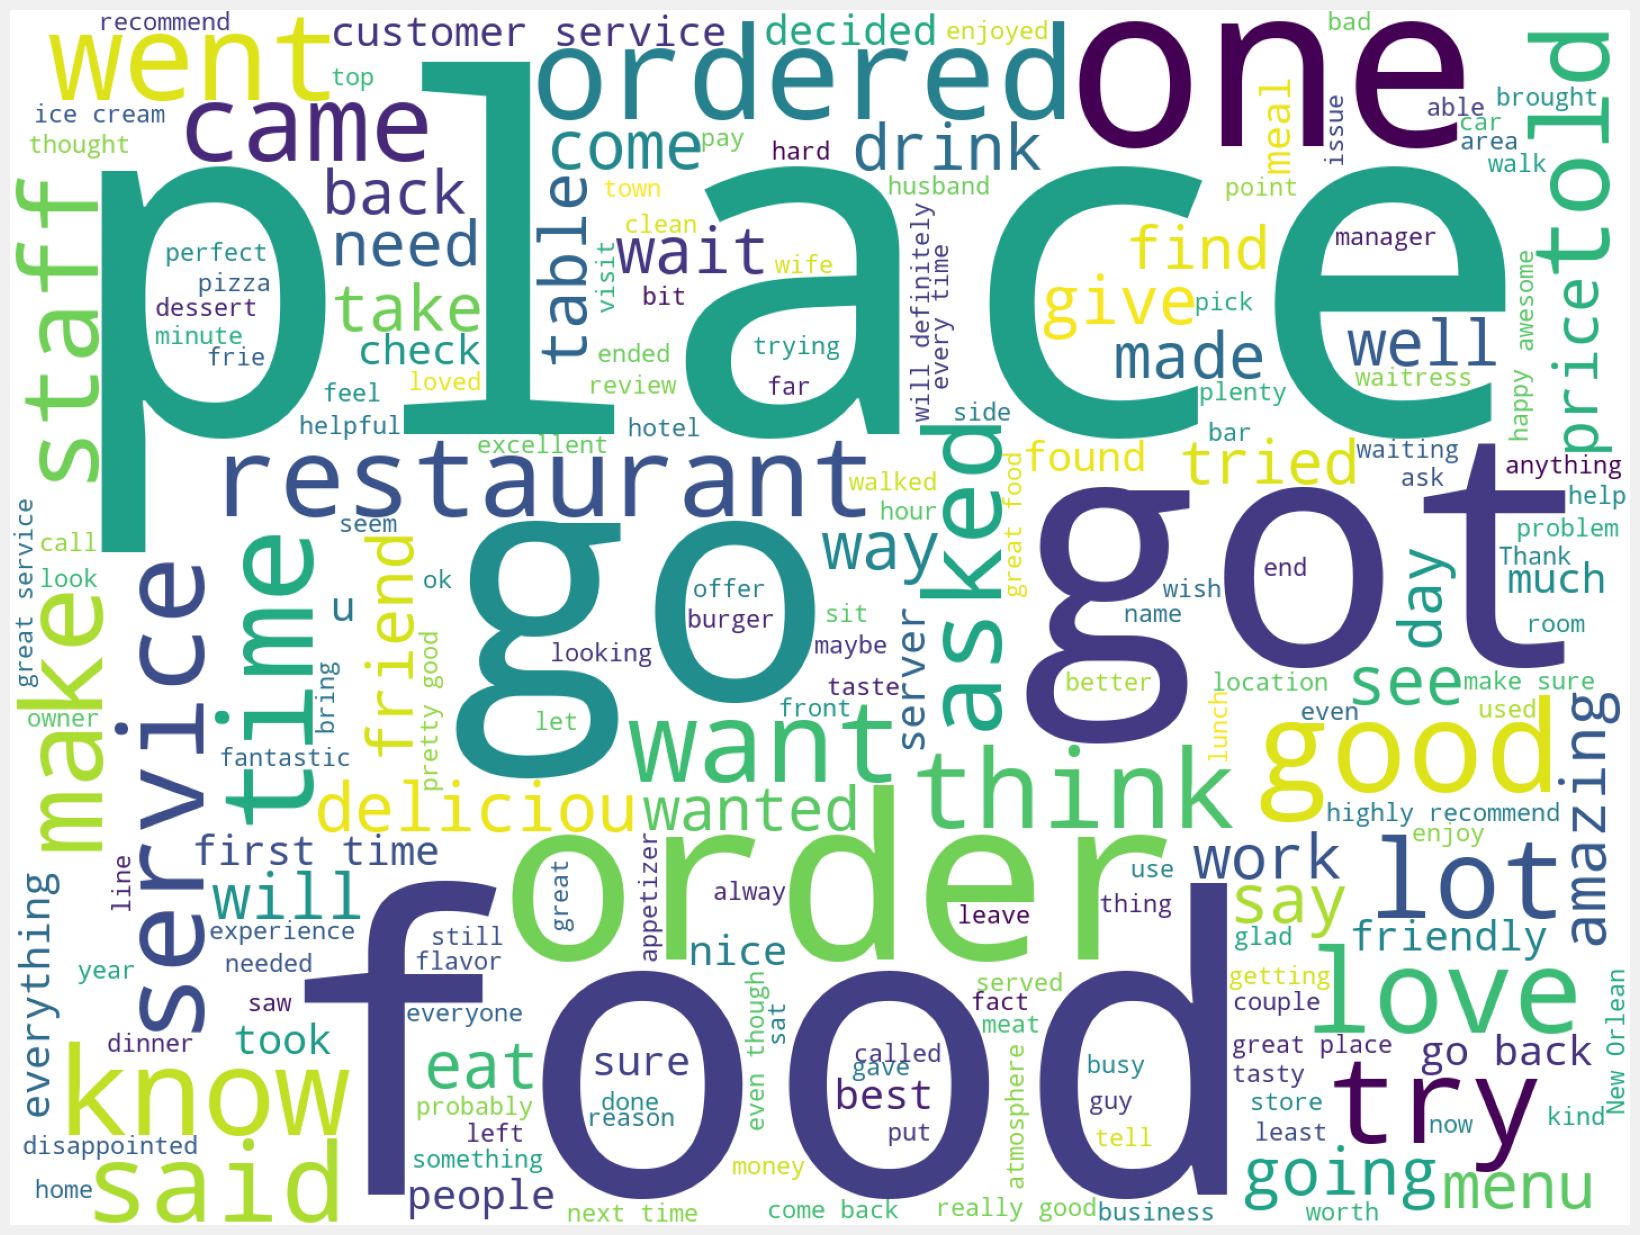
\includegraphics[width=0.47\textwidth]{figs/reviewWC.png}
        \label{fig:reviewwc}
    }
    \caption{Word Cloud Visualization of Categories and Reviews}
    \label{fig:combinedwc}
\end{figure}

\section{Data Collection}

\subsection{Web Crawler}

To enrich our original dataset, we utilize the web crawler to get up-to-date businesses from yelp.com. The target location is set in Singapore to meet our exploring interests in local business. To go through our web crawler in detail, 


The crawler is programmed to navigate through Yelp.com, targeting business listings within Singapore. It captures essential business details such as name, location, contact information, types of services or products offered, customer reviews, and ratings, etc. The YelpSpider class, a subclass from library 'scrapy.Spider', is the core of our crawler. It is initialized with parameters such as location, category, and starting\_num to target specific business listings in Singapore. The start\_requests method initiates the crawling process by building a URL using these parameters and sending a request to Yelp.com. Once the initial request is made, the parse method takes over, which navigates through the listings on Yelp. For each business listing encountered, it extracts the link to the detailed business page and makes a subsequent request to that page. This design ensures that we capture comprehensive details about each business.

Additionally, the crawler is equipped to handle pagination on Yelp's search results pages. It identifies the link to the next page (if present) and recursively calls the parse method to continue the extraction process until all relevant pages are covered. 

Since Yelp.com limits a maximum search result to 20 pages, we have to design an iterative method to "scan over" all the locations in Singapore. We first collected the list of all places (165 subzones in total) in Singapore from \href{https://en.wikipedia.org/wiki/List_of_places_in_Singapore}{Wikipedia} \cite{WikiListOfPlacesSG}, then ran our crawler script in each zone to perform the business collection locally.

The total crawling time was about 12 hours. Since there's some overlapping in each subzone, we applied uniqueness filtering at the post-processing step of the data crawling. In order to match the original form of business data, which benefits the crawled data fitting in the pipeline designed for the following steps, we also generate business\_ids from every unique URL via MD5 hashing. After removing duplicated data, we finally collected \textbf{6606 rows of business} in Singapore. 

We further visualize the crawled data of Singapore based on the analysis script described in section 2.2. Thanks to the great analysis notebook, we could interact with the result with different zoon-in levels\cite{OpenStreetMap}. The crawled business data is shown in figure \ref{fig:combined_map}, with each graph clustered by region. We chose the whole of Singapore, NUS, and Marina Bay as our regions of interest to visualize our crawled data.

\begin{figure}[!h]
    \centering
    \subfloat[Business in Singapore]{
        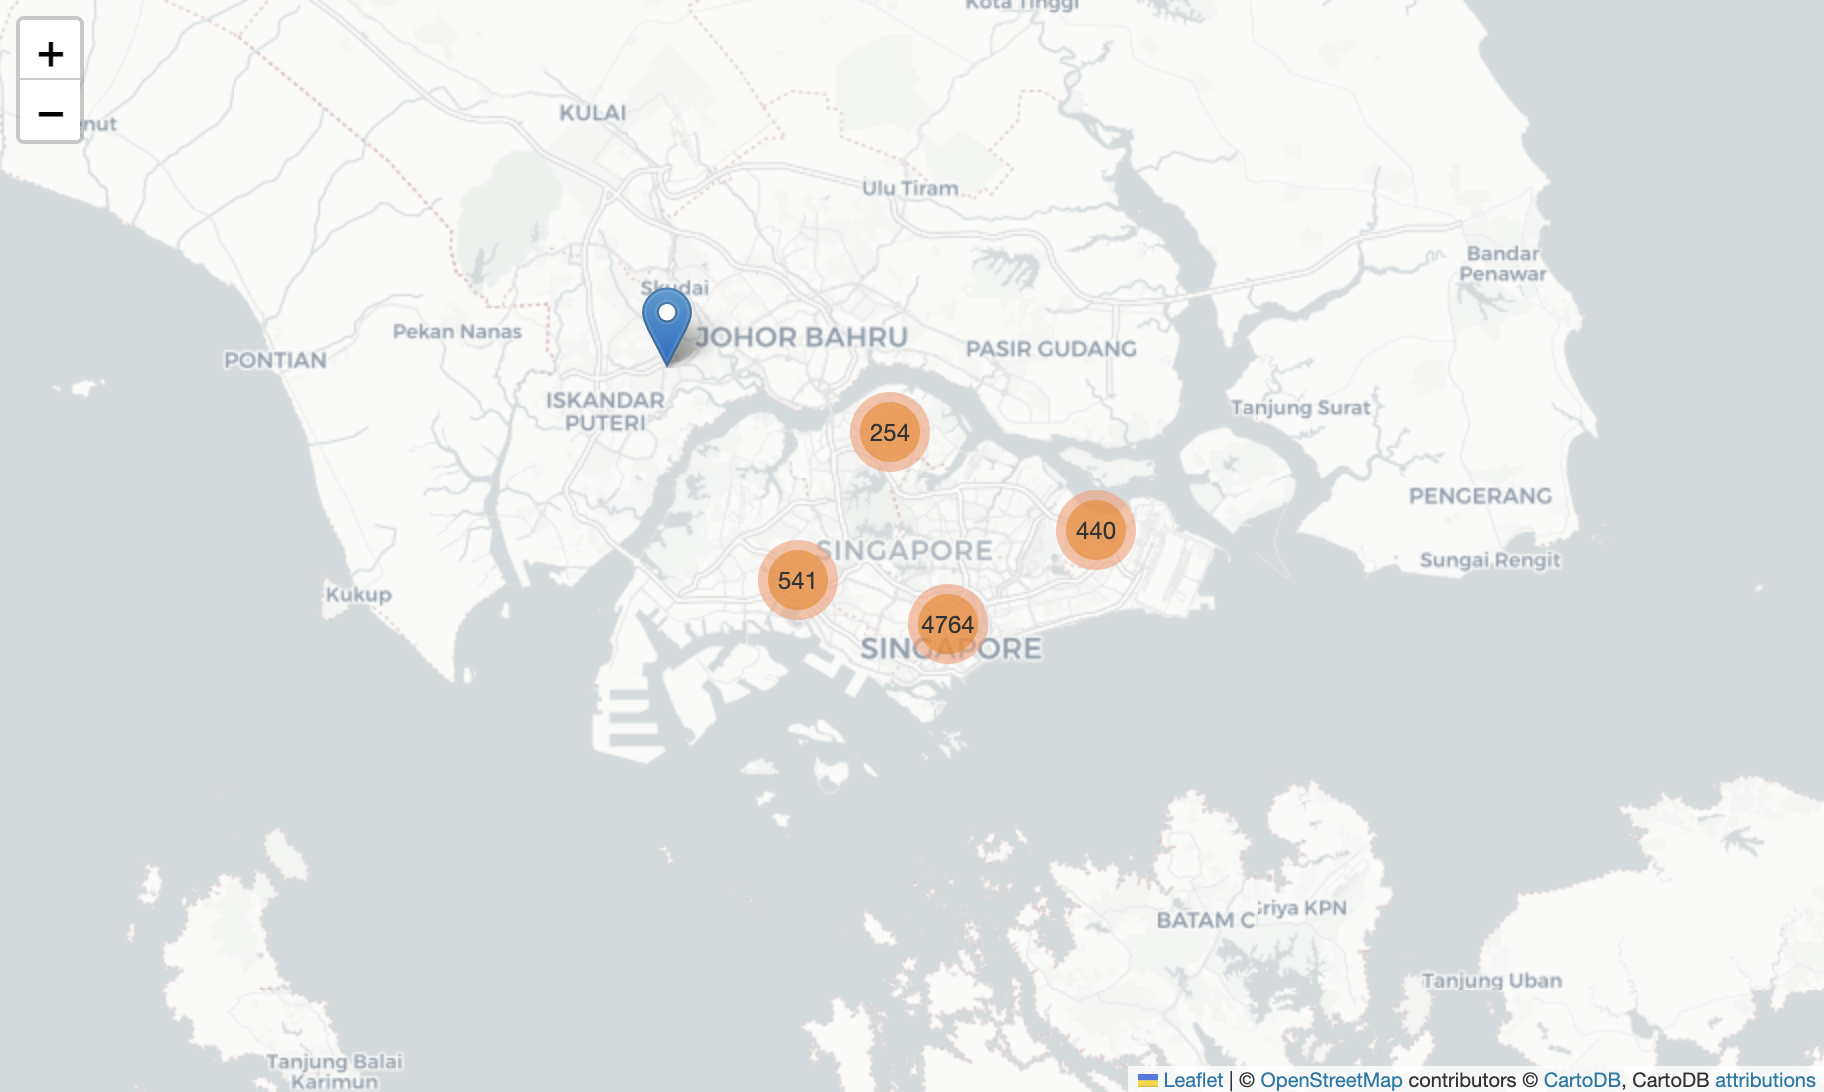
\includegraphics[width=0.47\textwidth]{figs/sg_map_zoom1.png}
        \label{fig:map1}
    }
    \hspace{0.07cm}
    \subfloat[Business in Singapore (Zoomed in)]{
        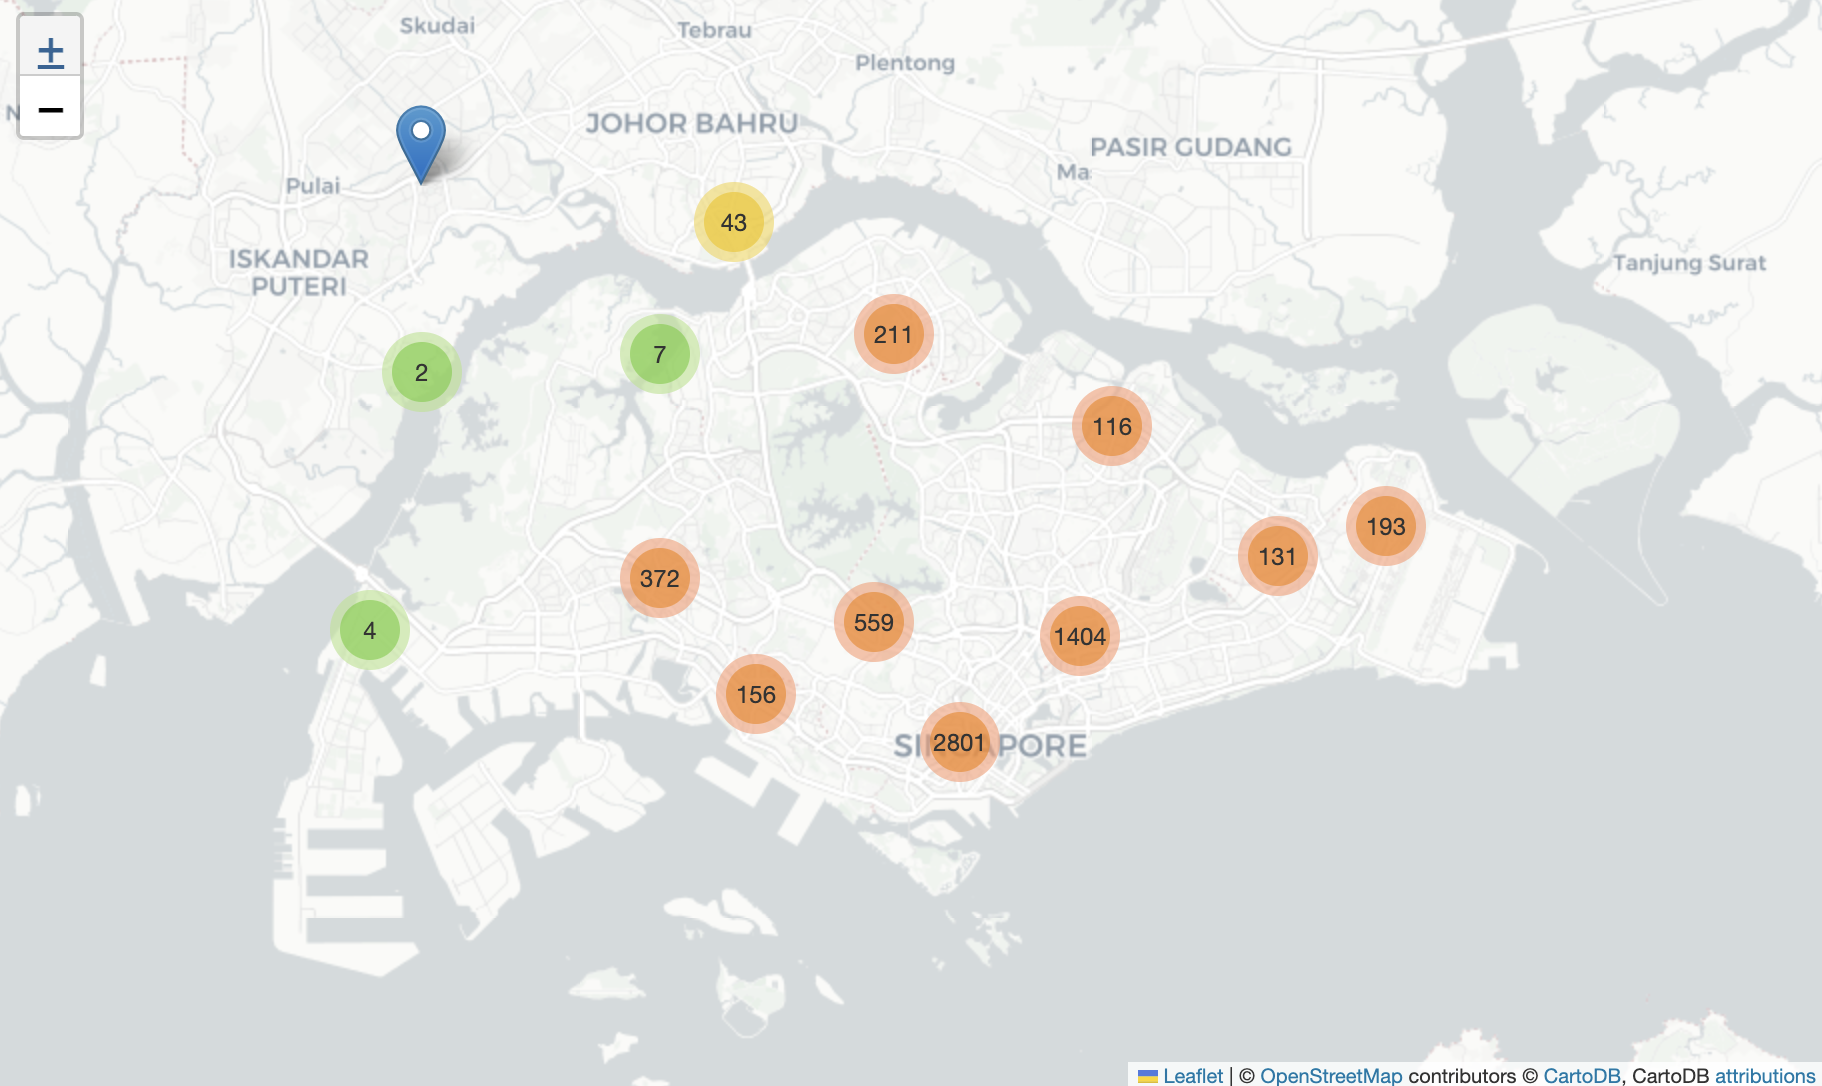
\includegraphics[width=0.47\textwidth]{figs/sg_map_zoom2.png}
        \label{fig:map2}
    }
    \vspace{0.0cm}
    \subfloat[Business around NUS]{
        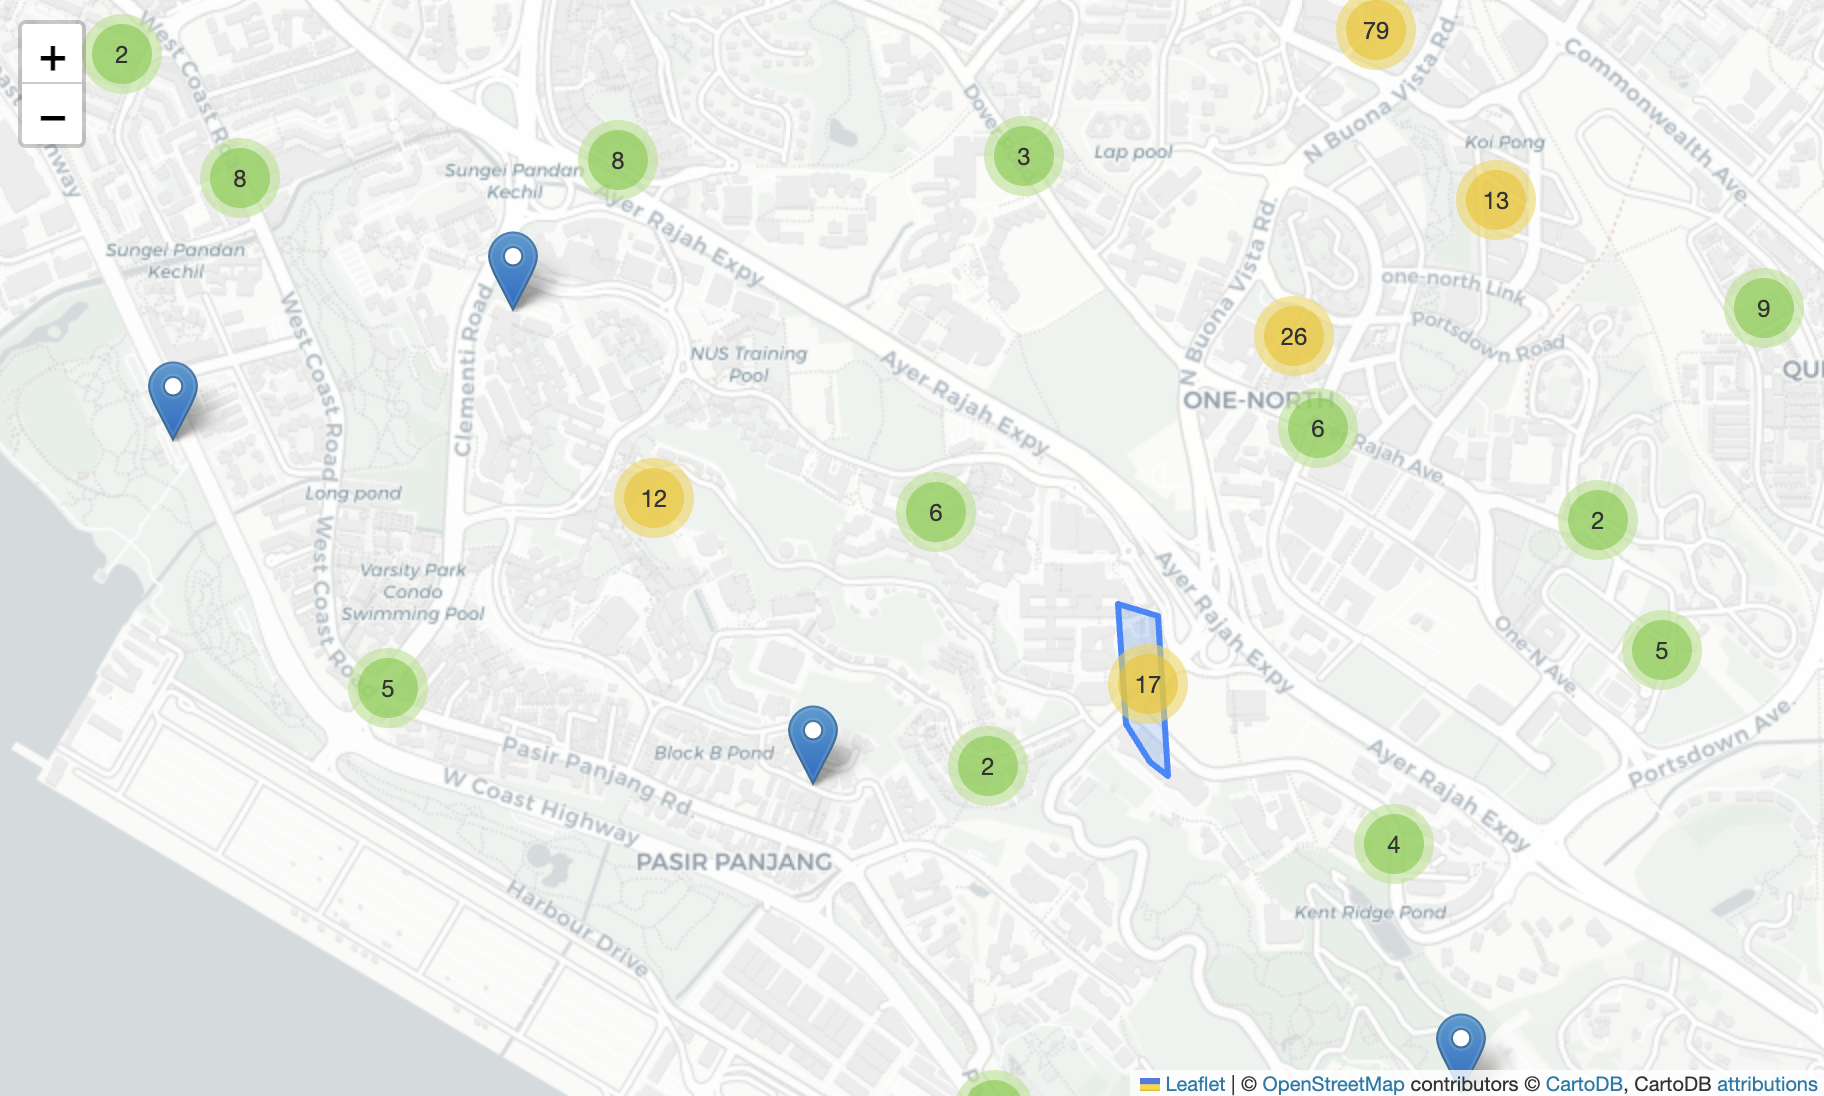
\includegraphics[width=0.47\textwidth]{figs/sg_map_zoom3.png}
        \label{fig:map1}
    }
    \hspace{0.07cm}
    \subfloat[Business around Marina Bay]{
        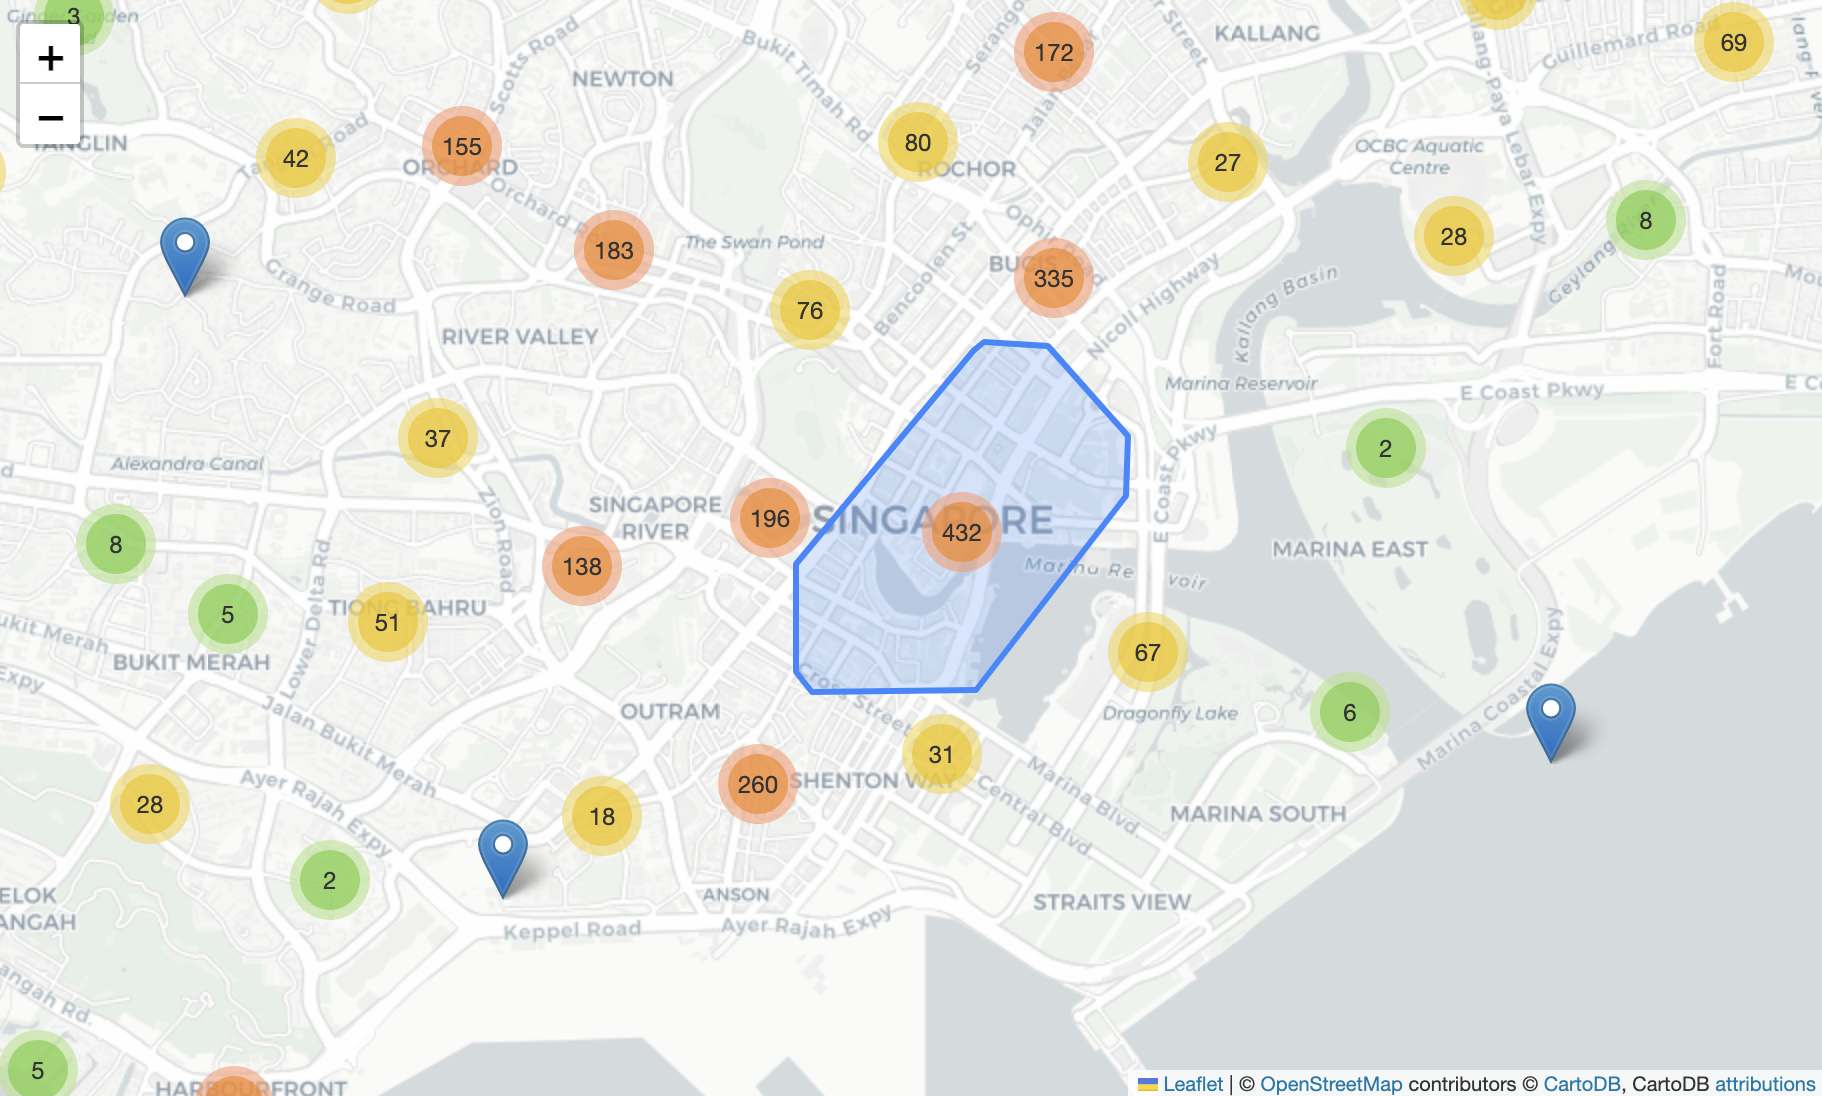
\includegraphics[width=0.47\textwidth]{figs/sg_map_zoom4.png}
        \label{fig:map2}
    }
    \caption{Different Locations in Singapore of Crawled Yelp Data}
    \label{fig:combined_map}
\end{figure}


\subsection{Large Language Model Generation}
To enrich our original dataset, we also apply some generative methods to perform data augmentation on the original dataset. Due to its robust and versatile capabilities, Large Language Models (LLMs) are extensively employed in a variety of scenarios. We leveraged their classification and generative abilities for conducting intriguing explorations and expansions of our dataset. Specifically, we used Llama-2 to perform data augmentation on \textbf{Transaction, Category Classification, and Review Analysis} on the original dataset.

\textbf{Llama-2}
Llama-2 is a collection of popular large language models open sourced by Meta, with state-of-the-art performance. These models are pretrained and fine-tuned generative text models ranging in scale from 7 billion to 70 billion parameters. For our specific task, we have selected 'Llama-2-7B-chat'.

\textbf{1. Transaction}
The 'check-in' table for each business includes only a series of check-in dates. Our approach involves generating an estimated transaction amount for each date. This will enable us to conduct detailed business analysis presentations using our database in this hypothetical scenario. We employed a technique that integrates random number generation with large language model creation to construct simulated trading scenarios.

Fig.\ref{fig:transaction} is an example of our generated transaction data. For all 131,929 business in 'check-in' table, we generated a total of \textbf{13,356,875} pieces of data.

\begin{figure}
    \centering
    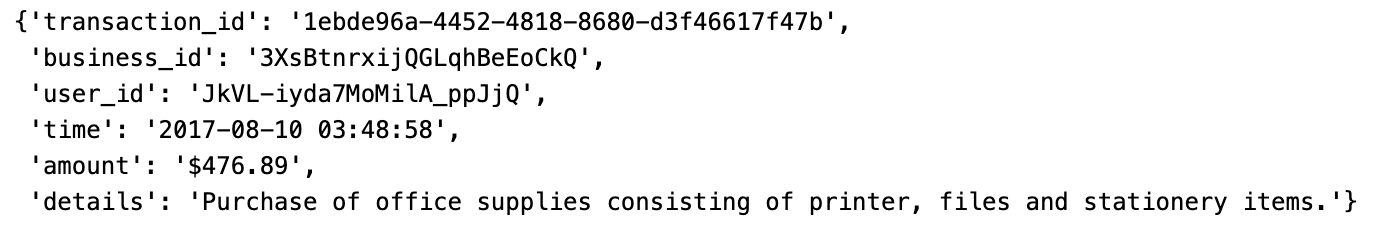
\includegraphics[width=1 \linewidth]{figs/transaction_example.png}
    \caption{Example of generated transaction data}
    \label{fig:transaction}
\end{figure}


\textbf{2. Category Classification}

We observed that the "categories" attribute in the "business" table contains disorganized original labels, making it challenging to isolate the specific business categories we need. To address this, we employed Llama-2 to assign each business a distinct category from the 36 categories we have meticulously designed.

For example, consider the initial "categories" attribute listing "Doctors, Traditional Chinese Medicine, Naturopathic/Holistic, Acupuncture, Health \& Medical, Nutritionists." This extensive and disorganized categorization poses challenges for practical applications, such as conducting category statistics and screening. To streamline this, we merged the 32 categories listed on the Yelp website with 4 additional ones, creating a total of 36 distinct categories. In the case of the aforementioned example, it would be aptly classified under the "Health" category.

We refined the original business table and generated a total of \textbf{60,000} data entries for application analysis. Fig.\ref{fig:category} displays the statistical outcomes for each category.

\begin{figure}
    \centering
    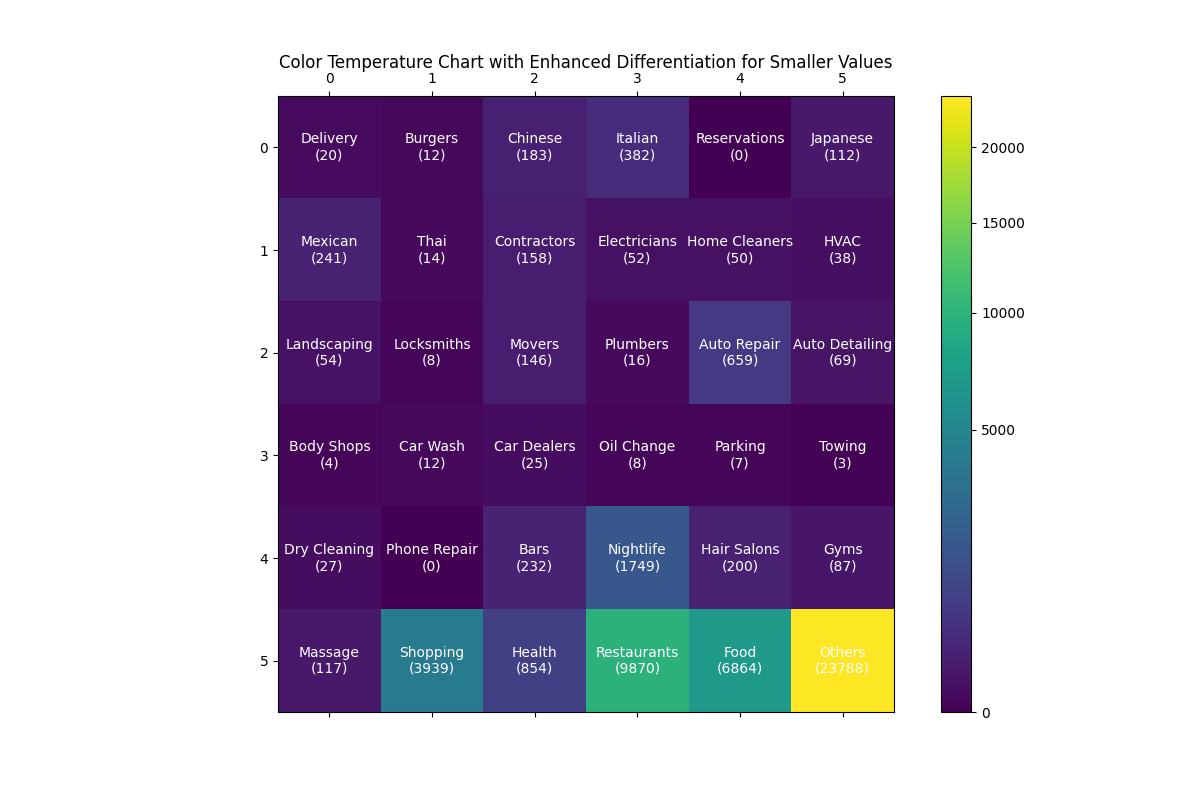
\includegraphics[width=1\linewidth]{figs/color_chart_categories.png}
    \caption{Generated category distribution map}
    \label{fig:category}
\end{figure}


\textbf{3. Review Analysis}

For the "texts" of user reviews in the "review" table, we can perform natural language processing (NLP) analysis to gain deeper insights. We noticed that on one hand, these reviews are imbued with highly subjective and personal emotions, while on the other, some offer meaningful insights, albeit others resemble mere running accounts. In response to this, we engaged in sentiment analysis and human-robot recognition tasks on these reviews, utilizing Llama-2.

We segmented sentiment analysis into five categories (1:Very Negative, 2:Negative, 3:Neutral, 4:Positive, 5:Very Positive), and Human-Robot Detection into two categories (1 for Human, 0 for Robot). To achieve this, we constructed specific prompts and employed a few-shot learning approach with Llama-2 to classify reviews. This process resulted in a total of \textbf{120,000} pieces of generated data.

For instance, for the first review "Sometimes this food is very very good. Unfortunately it's not consistent. Ordered something I've been getting for years and every other time it tastes incredible. It's like they have different people in the kitchen and you don't know who you will get. So 50 \% of the time it's excellent.", the model's generated rating results are "\{'sentiment': 3, 'human-robot': 1\}". This indicates that the model interprets this review as Neutral and authored by an actual Human.

Furthermore, to validate the effectiveness of our approach, we computed the Mean Squared Error (MSE) and Mean Absolute Error (MAE) between the sentiment analysis scores generated by our method and the star ratings provided by users. We discovered that both metrics were approximately \textbf{0.68}, indicating that our method is effective. This is because it closely aligns with the subjective scores directly given by users, while our analysis is fundamentally based on the content of the user reviews themselves.




\section{Data Storage}

% \subsection{Used Container Databases}

\subsection{Schema Design in MySQL}

\textbf{\\4.1.1 Schema Design and Diagram\\}

In the initial phase, we focused on data-centric aspects in designing the relational database. The attached figure \ref{fig:sch1} illustrates this initial design. However, upon further analysis, we identified several key deficiencies of simple design:

\begin{figure}[!h]
\centering
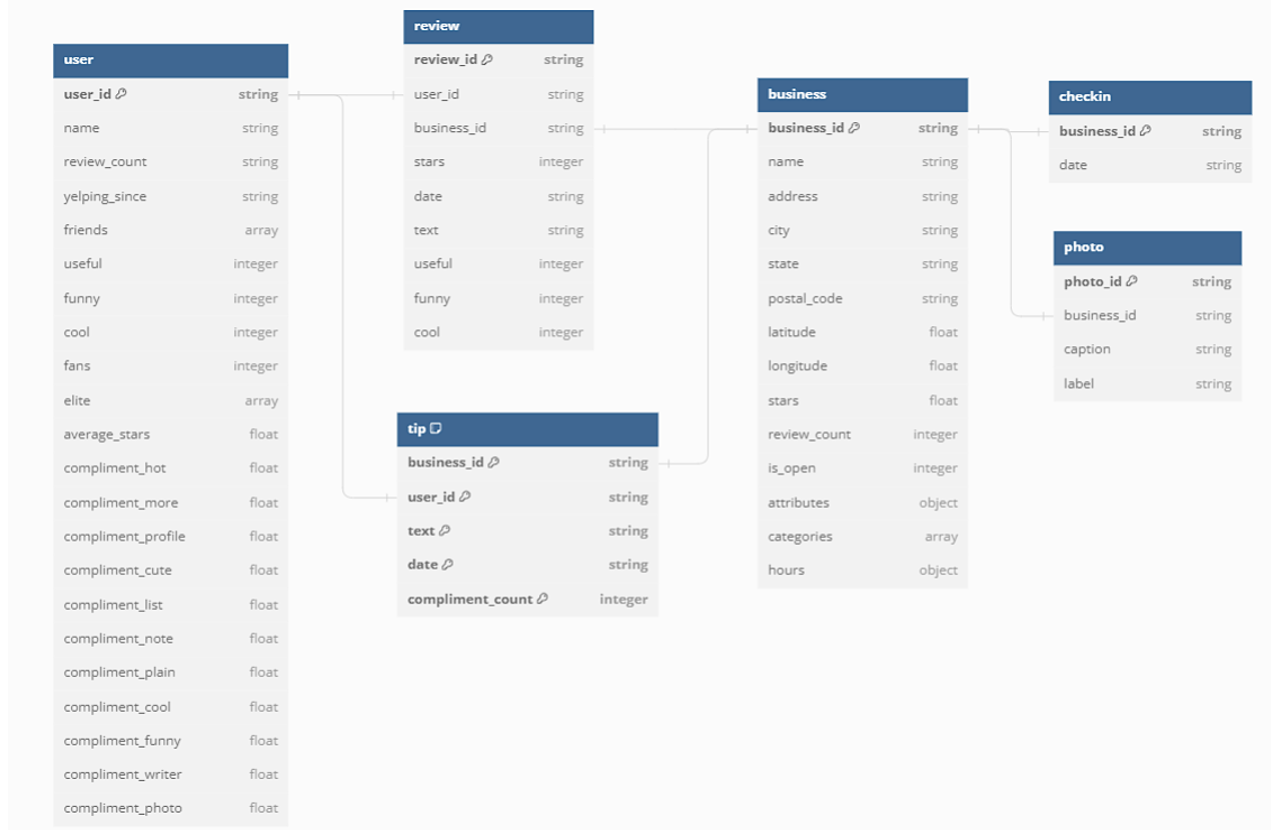
\includegraphics[height=8cm]{figs/schema_1.png}
\caption{Initial Design of our Schema}
\label{fig:sch1}
\end{figure}


\begin{itemize}
    \item Data Storage in JSON Files: A significant portion of our data is stored in JSON files, often as arrays or collections. This format, while flexible, poses challenges for efficient querying and data retrieval.

    \item Many-to-Many Relationships: The database design includes numerous many-to-many relationships between tables. This approach has led to considerable data redundancy, which not only consumes extra storage space but also complicates data management.

    \item Query Efficiency: The current design lacks optimization for query efficiency. This oversight can result in slower data retrieval times, impacting the overall performance of the database system.

    \item Compliance with BCNF (Boyce-Codd Normal Form): There is an absence of a thorough evaluation to determine if the database structure adheres to the BCNF constraints. Compliance with BCNF is crucial for reducing redundancy and ensuring data integrity.   
\end{itemize}


To summarize these, while the initial database design addresses basic data storage needs, it falls short in terms of query efficiency, data normalization, and optimal utilization of storage resources. A reevaluation and restructuring of the database schema are recommended to address these issues.

Subsequently, our team focused on optimizing the relational database structure in MySQL, informed by an in-depth analysis of the data structure. The revised design strategically divides different types of data into different tables to improve organization and efficiency. Business-related information is now stored only in the "Business" table, while user-related data is assigned to the "Users" table. Similarly, we have designated the "Review", "Check-ins" and "Photos" tables to store comments, check-ins and photo data respectively. In addition, we introduced the "Tips" and "Transactions" tables to manage tip-related information and transaction data. An important improvement in our redesign is the creation of a specialized "Friends" table, which is dedicated to encapsulating friend relationships between users. This optimized structure of the relational database is intended to simplify data management and improve the efficiency of the database system. An illustration of the optimized relational database design is shown in figure \ref{fig:sch2}.

\begin{figure}[!h]
\centering
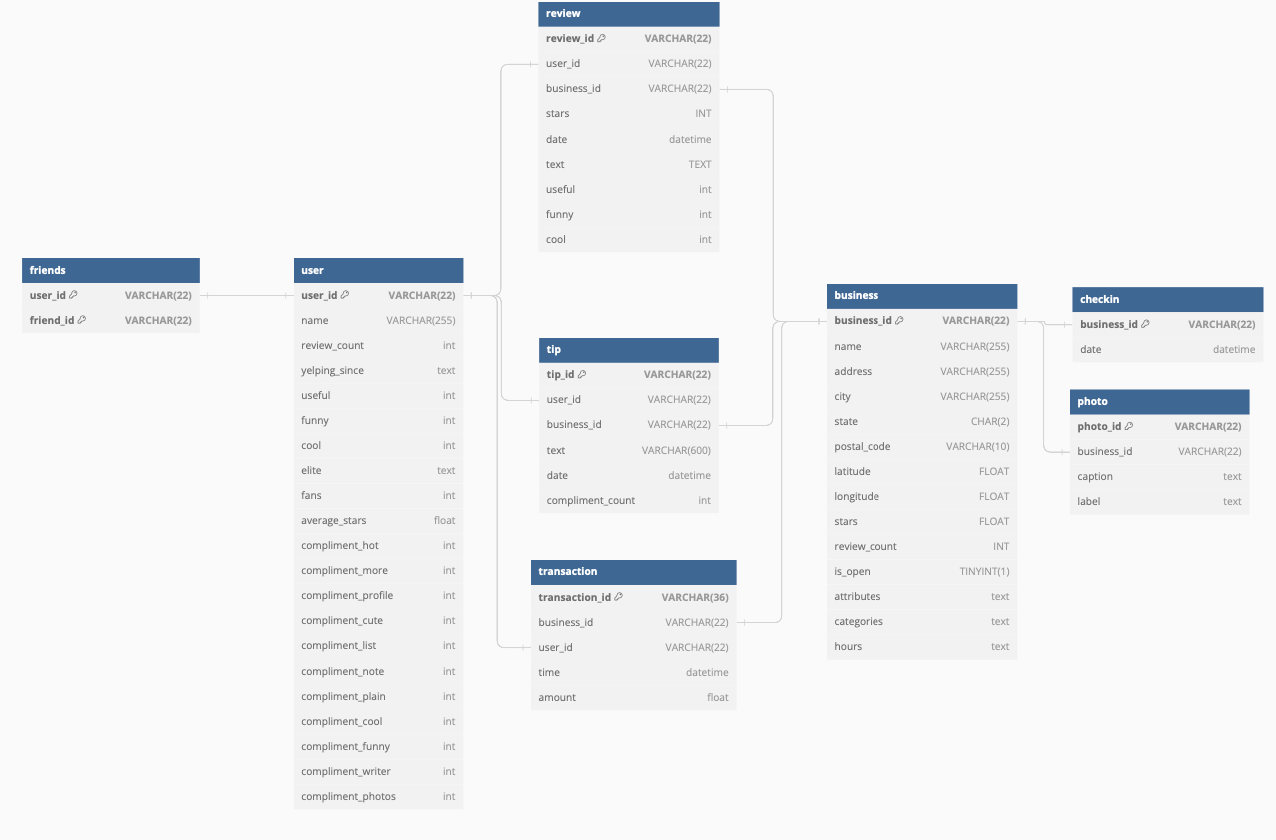
\includegraphics[height=8cm]{figs/schema_2.png}
\caption{Final Design of our Schema}
\label{fig:sch2}
\end{figure}

Our database system is designed to meet the needs of different user roles, providing users, business owners, and platform administrators with rich functions to serve a variety of application scenarios.


\textbf{\\4.1.2 Storage Logic\\}

Through the above table design, we are able to efficiently store and retrieve information related to business, users, reviews, etc. Associations between tables are established by foreign keys, ensuring data integrity and consistency. This approach not only enhances the relational database's organization but also facilitates effective data management and retrieval. We list our storage logic for MySQL database as follows:

Service data storage: The business table contains basic information about services, including the address, latitude and longitude, and star rating. The attributes, categories, and hours fields use text types to store JSON data.

User data storage: The User table contains basic information about the user, as well as a series of statistics related to the user, such as the number of likes, followers, etc.
review data storage: The review table stores users' comments on services, including ratings and dates.

Check-in data store: The checkin table stores the check-in records of users for a service, including the date and time.

Photo data storage: The Photo table stores photos uploaded by users, including photo descriptions and classifications.

Tip data storage: The Tip table stores user prompt information about services, including the date and number of likes.

Transaction data storage: The transaction table stores the transaction records of a user in a business, including the date, time, and amount.

\textbf{\\4.1.3 Advantages and Disadvantages\\}

\textbf{Advantages}: The structure of the database is clear, conforms to the design principle of the database paradigm, avoids data redundancy, and establishes the association between tables by using foreign keys to ensure the consistency of data.

\textbf{Cons}: For some business attributes, such as attributes, categories, and hours, storing JSON data using text types may require additional parsing at query time, may affect query performance, and may require regular maintenance of the table structure, especially if business requirements change.



\subsection{Collection Design in MongoDB}

\textbf{4.2.1 Non-relational Design Overview\\}

MongoDB's design is similar to MySQL in that it uses Collection instead of tables. Each Collection corresponds to a different set of data for business, users, reviews, and so on.
In particular to enhance query performance, MongoDB allows indexing on any document's field or subfield. This approach to indexing is notably different from MySQL’s, primarily due to MongoDB’s schema-less nature, which provides more flexibility but also requires careful index management to optimize performance. 

This is particularly useful in collections with high query demands, such as those storing user reviews, check-ins, and transaction data. Indexing these critical fields, such as date elements in review and transaction collections, significantly speeds up search and sorting operations. 

\textbf{\\4.2.2 Storage Logic\\}

In MongoDB, data storage is handled through collections, each serving a specific purpose similar to tables in MySQL. Understanding the storage logic in MongoDB, especially in comparison to the more traditional relational model of MySQL is crucial for effective database design. For each collection, here we provide a brief explanation of why its structure is beneficial in MongoDB’s document model compared to the relational model of MySQL.

User data storage: The user collection, similar to the User table in MySQL, holds basic user information along with user-related statistics. MongoDB’s document model enables the storage of these statistics in a more dynamic and scalable manner compared to the rigid structure of MySQL.

Review data storage: the review collection of MongoDB stores user comments on services, paralleling the review table int'm MySQL.

Check-in data storage: Check-in collection stores the check-in records of users on certain services, which corresponds to the Check-in table in MySQL.

Tip data store: the Tip collection stores user information about services and corresponds to the TIP table in MySQL.

Transaction data storage: the transaction collection stores the transaction records of users in a certain business, which corresponds to the transaction table structure in MySQL.

\textbf{\\4.1.3 Advantages and Disadvantages\\}

\textbf{Advantages}: MongoDB supports the storage of unstructured data and adapts to complex json structures such as categories and attributes in business data. Its data model is more flexible and can better respond to changes in business requirements.

\textbf{Cons}: In some scenarios that require complex queries, it may be necessary to write more aggregation pipelines to achieve complex queries, and there are some limitations in constraint support in MongoDB compared to MySQL for scenarios that require strict constraints.

\textbf{\\4.2.3 Summary of Database Design\\}

Our database design has been successful in meeting the needs of different application scenarios. Through reasonable table structure and index design, we can store and retrieve data efficiently, while ensuring data integrity and consistency. The design of application scenarios and tasks takes into account the requirements of different user roles, and provides rich functions and flexible query methods. Database systems can support large-scale data storage and efficient queries, providing powerful tools and functions for businesses, users, and administrators.

\subsection{Efficient Data Warehousing}

When loading cleaned JSON data into MySQL, we experimented with two different approaches. Initially, we attempted to read each document from the JSON file one by one and input the data line by line into the corresponding tables we had created in MySQL. However, due to the substantial size of our JSON file, this method proved to be highly time-consuming.

Subsequently, we adopted an alternative strategy, wherein we employed a chunking mechanism to read the JSON file in segments. We utilized the chunksize parameter along with pandas data frames to store the data temporarily. Then, leveraging the SQLAlchemy engine, we efficiently transferred the entire dataset into the MySQL database. This approach significantly enhanced the efficiency of the data loading process. The approximated data loading time are given in Table~\ref{table:headings}.


\setlength{\tabcolsep}{4pt}
\begin{table}
\begin{center}
\caption{Comparisons of Execution Time via Different Loading Methods.}
\label{table:headings}
\begin{tabular}{c|c|c}
\hline\noalign{\smallskip}
{\bf Loading Method} & {\bf Dataset} & {\bf Execution Time (Approx.)}\\
\noalign{\smallskip}
\hline
\noalign{\smallskip}
PyMySQL + Line by line & business & 1 hour
\\
PyMySQL + Line by line & friends & 10 hours +
\\
\noalign{\smallskip}
\hline
\noalign{\smallskip}
SQLAlchemy + Chunksize & business & 30 seconds
\\
SQLAlchemy + Chunksize & friends & 1 hour, 10 minutes
\\
\hline
\end{tabular}
\end{center}
\end{table}
\setlength{\tabcolsep}{1.4pt}

\section{Application Scenarios and Tasks}

\textbf{Application Overview:} Aiming at providing services for customers, business owners and platform administrators, the proposed application of our database is divided into following 3 scenarios:

\subsection{For Customers}

\textit{The most general and widely-used functions of our database. These applications provide some general information about the businesses for individuals, and could enhance the individual's experience through personalized and relevant data.}


\begin{enumerate}

    \item Get top-n businesses in the city n=10, 20, 50, 100

    \begin{itemize}
        \item[\textbullet] Detail: Rankings are based on a composite score considering factors like ratings, review counts, and customer feedback.
    \end{itemize}
    
    \item Get top-10 businesses within a specified radius m=0.1, 0.5, 1, 5, 10 km

    \begin{itemize}
        \item[\textbullet] Detail: Uses geolocation data (latitude, longitude) to find businesses in proximity.
    \end{itemize}


    \item Retrieve all reviews for a specific business by "business\_id", sorted by "stars"

   \begin{itemize}
        \item[\textbullet] Detail: Sorts reviews in descending order of star ratings, offering a quick overview of the most favorable customer feedback.
    \end{itemize}
    

    \item Access and update the user's own profile
    
    \begin{itemize}
        \item[\textbullet] Detail: Allows users to view and modify their personal information, including name, reviews, likes, etc.
    \end{itemize}

    \item View reviews of friends, sorted by datetime
    
    \begin{itemize}
        \item[\textbullet] Detail: Integrates social connections to display recent activity of friends, enhancing the social aspect of the platform.
    \end{itemize}

    \item Access recent reviews from influencers
    
    \begin{itemize}
        \item[\textbullet] Detail: Focuses on providing insights from reputable sources such as elite or popular users.
    \end{itemize}

\end{enumerate}




\subsection{For Business Owners}

\textit{Features for business owners focus on providing insights into customer behavior and relative business trends, with a strong emphasis on data privacy and sensitive information control across businesses and users.}




\begin{enumerate}

    \item Retrieve check-in histories for their business

    \begin{itemize}
        \item[\textbullet] Detail: Enables business owners to analyze customer visit patterns over time, aiding in business planning.
    \end{itemize}
    
    \item Access partial customer information

    \begin{itemize}
        \item[\textbullet] Detail: Provides essential customer data while maintaining strict adherence to privacy regulations.
    \end{itemize}


    \item Analyze time-series data for peak and off-peak times
    
   \begin{itemize}
        \item[\textbullet] Detail: Time-series characteristic retrieval. Assists in identifying business rush hours for better staffing and resource management.
    \end{itemize}
    

    \item Obtain average sentiment value from reviews within duration: 1, 7, 30 days
    
    \begin{itemize}
        \item[\textbullet] Detail: Uses sentiment analysis to rate customer reviews, offering insights into overall customer satisfaction. 
        \item[\textbullet] Note: sentiment values are scores varying from 0 to 5, generated by LLM
    \end{itemize}

    \item Access transaction records within the duration specified
    
    \begin{itemize}
        \item[\textbullet] Detail: Provides detailed financial transaction data for specified periods, aiding in financial management and analysis. 
        \item[\textbullet] Note: transaction data are simulated based on the real review data.
    \end{itemize}

\end{enumerate}




\subsection{For Platform Administrators}

\textit{For the most advanced tracking throughout businesses and customers. All functions are yielded with the highest accessibility. Provide YELP administrators with a toolbox for handling and maintaining the entire platform.}



\begin{enumerate}

    \item Identify active users within a specified period

    \begin{itemize}
        \item[\textbullet] Detail: Focuses on users who have engaged with the platform, particularly through reviews, in a given timeframe.
    \end{itemize}
    
    \item Detect robot-generated feedback
    \begin{itemize}
        \item[\textbullet] Detail: Employs advanced algorithm(LLM) to identify and filter non-human interactions and feedback.
        \item[\textbullet] Note: robot-generated values are scores in 0 or 1, generated by LLM
    \end{itemize}


    \item Analyze average business ratings across categories or regions
    
   \begin{itemize}
        \item[\textbullet] Detail: Provides a macro view of business performance across various sectors and geographical areas.
    \end{itemize}
    

    \item Find out influencers: Identify top-1000 popular users
    
    \begin{itemize}
        \item[\textbullet] Detail: Ranks users based on the sum of ratings like useful, funny, and cool, highlighting influential platform participants.
    \end{itemize}


\end{enumerate}


\section{Implementation and Performance Analysis}

\subsection{SQL Queries in MySQL}
\begin{enumerate}
    \item Get top-n businesses in the city n=10, 20, 50, 100
    \begin{verbatim}
    SELECT * FROM business WHERE city = 'Philadelphia' 
    ORDER BY stars
    DESC LIMIT 100;
    \end{verbatim}

    
    \item Get top-10 businesses within a specified radius m=0.1, 0.5, 1, 5, 10 km

    \begin{verbatim}
    SELECT * FROM business 
    WHERE SQRT(POW((latitude - (39.9298)), 2) + 
                POW((longitude - (-85.984)), 2)) * 111.32 <= 1  
    ORDER BY stars 
    DESC LIMIT 100;
    \end{verbatim}
    
    \item Get all reviews for a specific business, sorted by stars
    \begin{verbatim}
    SELECT * FROM review 
    WHERE business_id = (SELECT business_id from business
        WHERE name = "West Side Kebab House") 
    ORDER BY stars 
    DESC LIMIT 10;
    \end{verbatim}
    
    \item Get and update user's own profile (e.g. reviews, likes, elite records etc....)
    \begin{verbatim}
    SELECT user_id, name, yelping_since FROM user 
    WHERE user_id = 'j14WgRoU_-2ZE1aw1dXrJg';

    UPDATE user SET useful = 520, funny = 520, cool = 520
    where user_id = 'j14WgRoU_-2ZE1aw1dXrJg';
    \end{verbatim}

    \item Get review of their own friends, sorted by datetime
    \begin{verbatim}
    SELECT c.* FROM review  c 
    JOIN friends f ON c.user_id = f.friend_id 
    WHERE f.user_id = ‘j14WgRoU_-2ZE1aw1dXrJg’ 
    ORDER BY c.date DESC LIMIT 20;
    \end{verbatim}

    \item  Get the recent review from influencers 
    \begin{verbatim}
    WITH RankedUsers AS (
    SELECT 
        u.user_id,
        PERCENT_RANK() OVER (ORDER BY u.fans) AS percentile_rank
    FROM user u
    WHERE (u.elite LIKE '%2016%' OR u.elite LIKE '%2017%' 
                                        OR u.elite LIKE '%2015%')
    )
    SELECT r.*
    FROM review r
    JOIN RankedUsers ru ON r.user_id= ru.user_id
    WHERE ru.percentile_rank > 0.7
    ORDER BY r.date DESC;
    \end{verbatim}

    \item Get all check-in histories of their specific business
    \begin{verbatim}
    SELECT * FROM checkin c 
    WHERE c.business_id = -QI8Qi8XWH3D8y8ethnajA;
    \end{verbatim}
    
    \item Get the most information of their customers 
    \begin{verbatim}
    SELECT u.user_id, u.name, u.review_count, u.yelping_since 
    FROM user u 
    WHERE u.user_id IN 
    (SELECT DISTINCT user_id FROM review 
    WHERE business_id = '9n-1LQLX3ntBfBtMwgSpig');
    \end{verbatim}
    
    \item Get the time-series characteristics (peak times and off-peak times) of their business
    \begin{verbatim}
    SELECT HOUR(date) hour, count(*) frequency FROM checkin 
    WHERE business_id = '-QI8Qi8XWH3D8y8ethnajA' 
    GROUP BY hour ORDER BY hour;
    \end{verbatim}

    \item Get average sentiment value from the review table within a duration
    \begin{verbatim}
    
    \end{verbatim}

    \item Get transaction records of their business within a duration
    \begin{verbatim}
    SELECT * FROM transaction 
    WHERE business_id =  
    (SELECT b.business_id FROM business b 
    WHERE b.name = "Zio's Italian Market")  AND
    time BETWEEN '2013-01-01' AND '2015-01-01';
    \end{verbatim}
    
    \item Get all active users within a duration
    \begin{verbatim}
    SELECT u.* FROM user u 
    WHERE u.user_id IN 
    (SELECT DISTINCT r.user_id FROM review r 
    WHERE r.date BETWEEN '2015-01-01' AND '2017-01-01') ;
    \end{verbatim}

    \item Average rating of businesses across different categories or regions.
    \begin{verbatim}
    SELECT city, AVG(stars) FROM business 
    GROUP BY city; 
    \end{verbatim}

    \item Filter out influencers: get top-1000 users with the most popularity
    \begin{verbatim}
    SELECT  u.*, (useful + funny + cool) as popularity 
    FROM user u 
    order by popularity 
    DESC
    LIMIT 1000;
\end{verbatim}


\end{enumerate}
\subsection{NoSQL Queries in MongoDB}
\begin{enumerate}
    \item Get top-n businesses in the city n=10, 20, 50, 100
    \begin{verbatim}
    db.business.find({ city: "Cityname” }).sort({ stars: -1 })\
    .limit(n);
    \end{verbatim}

    
    \item Get top-10 businesses within a specified radius m=0.1, 0.5, 1, 5, 10 km

    \begin{verbatim}
    var bulkOps = [];
    
    db.business.find({}).forEach(function(business) {
        var location = {
            type: "Point",
            coordinates: [business.longitude, business.latitude]
        };
        bulkOps.push({
            updateOne: {
                filter: { _id: business._id },
                update: { $set: { location: location } }
            }
        });
        if (bulkOps.length === 1000) {
            db.business.bulkWrite(bulkOps);
            bulkOps = [];
        }
    });
    if (bulkOps.length > 0) {
        db.business.bulkWrite(bulkOps);
    }
    db.business.createIndex({ location: "2dsphere" });
    let userLocation = { type: "Point", coordinates: [userLng, \
    userLat] };
    db.business.aggregate([
        {
            $geoNear: {
                near: userLocation,
                distanceField: "distance",
                spherical: true,
                maxDistance: m * 1000,
                query: { is_open: 1 } 
            }
        },
        {
            $limit: 10
        },
        {
            $project: {
                business_id: 1,
                name: 1,
                address: 1,
                distance: "$distance"
            }
        }
    ]);
    \end{verbatim}
    
    \item Get all reviews for a specific business, sorted by stars
    \begin{verbatim}
    var targetBusinessName = "business_name";
    var targetBusiness = db.business.findOne({ name:\
    targetBusinessName });  
    if (targetBusiness) {
        var targetBusinessId = targetBusiness.business_id;
        var reviewsForTargetBusiness = db.review.find({\
        business_id: targetBusinessId }).sort({ stars: 1 });

    \end{verbatim}
    
    \item Get and update user's own profile (e.g. reviews, likes, elite records etc....)
    \begin{verbatim}
    db.user.find({ user_id: "YourUserID" });
    db.user.update({ user_id: "YourUserID" }, { $set: \
    { /* Update fields */ } }); 
    \end{verbatim}

    \item Get review of their own friends, sorted by datetime
    \begin{verbatim}
    var targetUserId = "your_target_user_id";
    var targetUser = db.user.findOne({ user_id: targetUserId });
    if (targetUser) {
        var friendsList = targetUser.friends.split(",") : [];
        var friendsReviews = db.review.find({ user_id: { $in:\
        friendsList } }).sort({ date: 1 });
    } else {
        print("User not found with user_id: " + targetUserId);
    }
    \end{verbatim}

    \item  Get the recent review from influencers 
    \begin{verbatim}
    var currentYear = new Date().getFullYear();
    var threeYearsAgo = currentYear - 3;
    var eliteUserIds = db.user.find({
      $expr: {
        $and: [
          { $regexMatch: { input: "$elite", regex: new RegExp\
          (threeYearsAgo + "|" + (threeYearsAgo - 1) + "|" + \
          (threeYearsAgo - 2)) } },
          { $gt: ["$fans", 0] }
        ]
      }
    }).sort({ "fans": -1 }).limit(Math.ceil(0.3 * db.user.\
    countDocuments())).map(user => user.user_id);
    var recentInfluencerReviews = db.review.find({ \
    "user_id": { $in: eliteUserIds } }).sort({ "date": -1 })\
    .limit(10);
    \end{verbatim}

    \item Get all check-in histories of their specific business
    \begin{verbatim}
    db.checkin.find({ "business_id": “business_id” })
    \end{verbatim}
    
        \item Get the most information of their customers 
        \begin{verbatim}
    var businessUserIds = db.review.find({'business_id':\
    'XQfwVwDr-v0ZS3_CbbE5Xw'}, {'user_id': 1, '_id': 0}).\
    map(function(doc) {
        return doc.user_id;
    });
    var users = db.user.find({
        'user_id': { $in: businessUserIds } }, \
        { '_id': 0, 'user_id': 1, 'name': 1, \
        'review_count': 1, 'yelping_since': 1 });
    \end{verbatim}
    
    \item Get the time-series characteristics (peak times and off-peak times) of their business
    \begin{verbatim}
    db.transaction.aggregate([
        {
            $match: {
                "business_id": "XQfwVwDr-v0ZS3_CbbE5Xw" 
            }
        },
        {
            $project: {
                hour: { $hour: "$time" }
            }
        },
        {
            $group: {
                _id: "$hour",
                count: { $sum: 1 }
            }
        },
        {
            $sort: { count: -1 }
        },
    ]);
    \end{verbatim}

    \item Get average sentiment value from the review table within a duration
    \begin{verbatim}
    
    \end{verbatim}

    \item Get transaction records of their business within a duration
    \begin{verbatim}
    db.transaction.find({'business_id': 'D8y8ethnajA',\
    'date': {$gte: '2014-01-01',$lte: '2017-01-01'}},\
    {_id:0, business_id: 1, date: 1} )
    \end{verbatim}
    
        \item Get all active users within a duration
        \begin{verbatim}
    var startDate = ISODate("2010-06-07T22:09:11.000+00:00");
    var endDate = ISODate("2020-06-08T22:09:11.000+00:00");   
    const reviewUserIds = db.review.distinct("user_id", {
      "date": {
        $gte: startDate,
        $lt: endDate
      }
    });
    db.user.find({
      "user_id": { $in: reviewUserIds }
    }, { _id: 0, user_id: 1, name: 1 }) 
    \end{verbatim}

    \item Average rating of businesses across different categories or regions.
    \begin{verbatim}
    db.business.aggregate([
      {
        $group: {
          _id: "$categories", 
          average_rating: { $avg: "$stars" }
        }
      },
      {
        $sort: { average_rating: -1 } 
      }
    ]);
    \end{verbatim}

    \item Filter out influencers: get top-1000 users with the most popularity
    \begin{verbatim}
    db.user.aggregate([
      {
        $project: {
          user_id: 1,
          name: 1,
          popularity: { $sum: ["$useful", "$funny", "$cool"] }
        }
      },
      {
        $sort: { popularity: -1 }
      },
      {
        $limit: 1000
      }s
    ]);
\end{verbatim}


\end{enumerate}


\subsection{Running Time Comparison}

We report the execution time of each query as follows in table \ref{table:time}. To maintain a fair comparison, we conducted the execution of queries on the same device. The schema and collection design are implemented as described in the previous section. Please refer to Sections 5.1, 5.2, and 5.3 for query semantic details.

\setlength{\tabcolsep}{3pt}
\begin{table}[!h]
\begin{center}
\caption{Comparisons of execution time via different databases. Note that for each row, we calculated the percentage of MongoDB execution time over MySQL execution time.}
\label{table:time}
\begin{tabular}{c|c|c|c}
\hline\noalign{\smallskip}
{\bf No.} & \multicolumn{2}{c|}{\bf Implementation Database} & {\bf Ratio of Time Spent}\\
{\bf Query} & {\bf MySQL Time} & {\bf MongoDB Time}& {\bf MongoDB/MySQL (\%)}\\
\noalign{\smallskip}
\hline
\noalign{\smallskip}
1 & 0.53 sec & 0.13 sec & 24.53\% \\
2 & 0.33 sec & ~~0.001 sec \textit{*} & 0.30\% \\
3 & 2 min 6.45 sec & 19.48 sec & 15.38\% \\
4 & 2.55 sec & 0.001 sec & 0.04\% \\
5 & 7 min 42.40 sec & ~~0.10 sec \textit{*} & 0.001\% \\
6 & 3 min 1.35 sec & ~~0.43 sec \textit{*} & 0.002\% \\
7 & 10.31 sec & 0.05 sec & 0.48\% \\
8 & 1 min 53.66 sec & 2 min 13.76 sec & 105.49\% \\
9 & 10.00 sec & 5.77 sec & 57.70\% \\
10 & - & 0.76 sec & - \\
11 & 26.32 sec & 20.65 sec & 78.46\% \\
12 & 2 min 30.05 sec & 2 min 55.87 sec & 117.21\% \\
13 & 0.43 sec & 0.38 sec & 93.02\% \\
14 & 3.54 sec & 1.97 sec & 55.65\% \\
\hline
\end{tabular}
\end{center}
\end{table}
\setlength{\tabcolsep}{1.4pt}

Please note that for queries with the symbol * in table \ref{table:time}, we either designed extra indexes, or pre-updated extra attributes to speed up the MongoDB execution. Thus there is a huge difference in execution time from MySQL.

\subsection{Database Performance Analysis}

From Table \ref{table:time}, we can generally observe:

\textbf{Faster Execution in MongoDB}: Queries 1, 2, 4, 5, and 6 showcase MongoDB's superior performance, attributed to its efficient handling of unstructured data and effective use of indexes. For instance, in Query 2, the Geospatial index of MongoDB greatly boosts the location-based querying.

\textbf{Exceptional Cases}: Queries 8 and 12, where MongoDB takes longer time, highlight scenarios where relational databases might perform better. This could be due to the nature of the query, which might be more suited to a structured query language or involve complex relations better handled by MySQL. For instance, Query 8 accesses partial customer information given a "business\_id", which involves a join-like operation between "business" and "reviews" as tables or collections. In this case, a relational database like MySQL may have a better performance than MongoDB.

\textbf{Special Considerations}: The marked improvement in MongoDB's performance for certain queries (marked with *) is due to additional optimizations like extra indexes or pre-updated attributes. However, these outperforming may basically come from \underline{\textbf{our optimization focus on the MongoDB side}}. It is worth pointing out that there may be possibilities for further optimization of MySQL as well, but since we will be using MongoDB in the web service demo, we have further emphasized the optimization of MongoDB.


To sum up our observation, MongoDB generally offers superior query performance in our cases due to its schema flexibility and efficient handling of unstructured data, but there are some complicated scenarios where a traditional relational database like MySQL may be more suitable. 

Moreover, we'd like to share some experiences found in developing this project. When working with data storage, we found that the flexibility of MongoDB makes it less work to do data entry, but relatively complex to maintain and write query. MySQL, on the other hand, requires a lot of integrity constraints to be added when performing data storage, which is a relatively large amount of designation work, but is easier to maintain the database later.

\section{Prototype Demo}

\subsection{Backend Design}

In our prototype, the backend is structured around three core components: MongoDB, Flask \cite{grinberg2018flask}, and PyMongo. MongoDB serves as our database (DB), Flask acts as the request server, and PyMongo is utilized as the Database Management System API (DBMS API). To achieve a robust backend, Flask and PyMongo are integrated into a unified Python script. This integration enables a unified interaction between the database and the server.

Key functionalities implemented in the backend include the queries and corresponding parameters we defined above, each of which is accessible through specific API requests. We design our APIs following RESTful principles \cite{RichardsonRuby07} to making it easier for frontend components to interact.

\subsection{Frontend Design}

We implemented a Vue-based front-end website to interact with our Yelp Insight database platform, making it simple to interact and retrieve the data with visualization. The details of our interactive front-end design will be released together with the demo. See the "demo" directory under our project GitHub directory (\url{https://github.com/Linlt-leon/Yelp-Insight}) for more details.


\section{Conclusions}

In this project, we proposed a comprehensive data platform, namely \textit{Yelp Insight}, for customers, business owners, and administrators. The main contribution of our project can be concluded as follows: 1. We added more than 6,000 entries of Yelp data using the customized web crawler, and 180,000 rows of features via large language model generation techniques. 2. We carefully explored the characteristics of our Yelp dataset and presented many interesting insights into Yelp. 3. We provide more than 100 querying methods via the combination of our 16 basic queries and flexible parameters, which could cover a wide range of demands from customers, business owners, and platform administrators. 4. We built a demo website that can provide data access services via a non-coding interface. We believe the presented Yelp Insight well covers all aspects of the project tasks.

\clearpage
% ---- Bibliography ----
%
% BibTeX users should specify bibliography style 'splncs04'.
% References will then be sorted and formatted in the correct style.
%
\bibliographystyle{splncs04}
\bibliography{egbib}


% yelp
% SQL
% MongoDB
% https://en.wikipedia.org/wiki/List_of_places_in_Singapore

% \clearpage

% \appendix
% \section*{Appendix}
% We present more


\end{document}
